\documentclass[a4paper,12pt,titlepage]{article}
\usepackage[utf8]{inputenc}
\usepackage{graphicx} % Required for inserting images
\usepackage[spanish,es-tabla]{babel}
\usepackage[none]{hyphenat}
\usepackage[justification=centering]{caption}
\usepackage{subcaption}
\usepackage{amssymb, amsmath}
\usepackage{gensymb}
\usepackage{fancyhdr}
\usepackage{wrapfig}
\usepackage{physics}
\usepackage[table,xcdraw]{xcolor}
\usepackage{hyperref}

\usepackage[a4paper]{geometry}
\geometry{top=3cm, bottom=3.0cm,left=2cm, right=2cm}


\lhead{Circuito RLC paralelo}
\rhead{Gonzalo Bastos González}

\pagestyle{fancy}

\title{Circuito RLC paralelo - Análisis de Fourier}
\author{Gonzalo Bastos González}
\date{Técnicas expermimentales II-Laboratorio de electromagnetismo}

\begin{document}

\maketitle
\tableofcontents

\newpage

\section{Objetivos}

El objetivo de esta práctica es el estudio del comportamiento de un circuito RLC conectado en paralelo. El estudio de estos circuitos es interesante por su aplicación como filtro de las señales, ya que da preferencia a las señales sinusoidales con frecuencias cercanas a la frecuencia de resonancia del propio circuito. Para el estudio del circuito en paralelo vamos a observar el comportamiento de diferentes señales periódicas al atravesar el circuito, obteniendo los armónicos de las diferentes señales, que estudiaremos mediante su desarrollo en series de Fourier.

\section{Introducción teórica}

\subsection{Circuito RLC}

Denominamos circuito RLC a aquel circuito eléctrico formado por resistencias, bobinas y condensadores. Las magnitudes que caracterizan estos tres componentes son la resistencia $R$, la inductancia $L$ y la capacidad $C$ respectivamente. Estos circuitos son especialmente importantes, pues presentan fenómenos de resonancia muy interesantes de estudiar. La resonancia es un fenómeno que se produce cuando la tensión aplicada y la intensidad de corriente que circula por el circuito están en fase, dando lugar a que el circuito sea capaz de generar voltajes y corrientes más altos que los que lo alimentan. La resonancia está estrechamente relacionada con el concepto de impedancia, que no es más que una extensión a los circuitos de corriente alterna del concepto de resistencia y viene dada por la siguiente expresión compleja:

\begin{equation}
    Z = R + j\left(\omega L - \frac{1}{\omega C} \right) = R + j\chi
\end{equation}

Donde $Z$ es la impedancia, $\chi$ es la reactancia y $j$ es la unidad imaginaria. El fenómeno de resonancia se da cuando la impedancia se reduce exclusivamente a una resistencia $R$, por lo que se debe cumplir que $\chi=0$. En nuestro caso tenemos dos reactancias: la reactancia inductiva $\chi_L$ y la reactancia capacitiva $\chi_C$. Para que la reactancia total se anule estas dos deben ser iguales en valor absoluto, $\chi_L=\chi_C$. Si aplicamos esta condición llegamos a la condición que debe cumplir la frecuencia de resonancia de nuestro circuito RLC:

\begin{equation}
    \left.\begin{array}{c}
    \chi_L = 2\pi f L   \\ \\
    \chi_C = \frac{1}{2\pi f C}
    \end{array} \right\}
    2\pi f_0 L = \frac{1}{2\pi f_0C} \Rightarrow f_0 = \frac{1}{2\pi \sqrt{LC}}
    \label{f0}
\end{equation}

Siendo $f_0$ la frecuencia de resonancia de nuestro circuito, que podemos ver que depende únicamente de las características del propio circuito. Si la frecuencia de la señal de entrada es igual a la frecuencia $f_0$ entonces el desfase, $\phi$, entre la intensidad de la corriente alterna y la tensión es de $0^{\circ}$.

No obstante, para caracterizar totalmente nuestro circuito necesitamos dos magnitudes más, el ancho de banda y el factor de calidad. Por un lado lado tenemos el ancho de banda, que designa la longitud del intervalo de frecuencias que concentra la mayor potencia de la señal. Este intervalo está comprendido entre las frecuencias con desfase de $\pm 45^{\circ}$:

\begin{equation}
    B = f_{(\phi=45^{\circ})} - f_{(\phi=-45^{\circ})}
    \label{band_w}
\end{equation}

\newpage

Por otro lado, la última magnitud necesaria para caracterizar nuestro circuito es el factor de calidad, $Q$, que relaciona la energía almacenada con la energía disipada durante un ciclo completo de señal, cuanto más elevado es el factor $Q$ más agudo es el pico de resonancia. El factor de calidad se encuentra directamente relacionado con el ancho de banda:

\begin{equation}
    Q = \frac{f_0}{B}
    \label{q_factor}
\end{equation}

\begin{figure}[h!]
    \centering
    \begin{subfigure}{0.45\textwidth}
        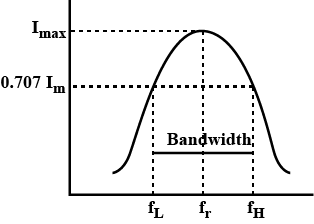
\includegraphics[width=0.95\linewidth]{fourier/band_width.png}
        \subcaption{Ancho de banda}
    \end{subfigure}
    \begin{subfigure}{0.45\textwidth}
        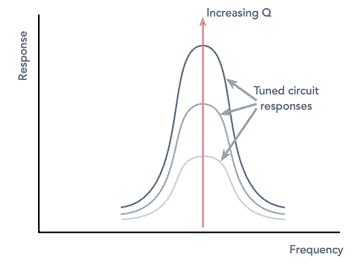
\includegraphics[width=0.95\linewidth]{fourier/q_factor.png}
        \subcaption{Factor de calidad}
    \end{subfigure}
    \caption{Magnitudes características del circuito RLC}
    \label{fig:enter-label}
\end{figure}

\subsection{Series de Fourier}

Para caracterizar el comportamiento de las señales empleadas vamos a emplear el desarrollo en serie de Fourier, que nos permite expresar cualquier función periódica como una suma infinita de funciones sinusoidales. Si consideramos una función $f(t)$ con período $T$ su desarrollo en serie de Fourier viene dado por la siguiente expresión:

\begin{equation}
    f(t) = \frac{a_0}{2} + \sum_{n=1}^{\infty} a_n \cos \left( \frac{2\pi n}{T} t \right) + b_n \sin \left( \frac{2\pi n}{T} t \right)
\end{equation}

Donde $a_0$, $a_n$ y $b_n$ son los coeficientes de Fourier, que se pueden calcular a partir de las siguientes integrales:

\begin{equation}
    \begin{gathered}
    a_0 = \frac{2}{T} \int_{-T/2}^{T/2} f(t) \dd t \quad a_n = \frac{2}{T} \int_{-T/2}^{T/2} f(t) \cos \left(\frac{2\pi n}{T}t\right) \dd t \\ b_n = \frac{2}{T} \int_{-T/2}^{T/2} f(t) \sin \left(\frac{2\pi n}{T}t\right) \dd t
    \end{gathered}
\end{equation}

Esta serie de Fourier está expresada en términos del período de la onda, pero podemos expresarla en función de la frecuencia $\omega$ de la onda a partir de la relación $\omega=2\pi/T$:

\begin{equation}
    f(t) = \frac{a_0}{2} + \sum_{n=1}^{\infty} a_n \cos \left( n\omega t \right) + b_n \sin \left( n\omega t \right)
\end{equation}

Los coeficientes n-ésimos de la serie de Fourier se denominan armónicos de la serie y son los que observaremos durante el transcurso de la práctica, como detallaremos más adelante.

Además de eso, a la hora de estudiar el desarrollo de Fourier de las señales introducidas en el circuito es de gran importancia la paridad de las funciones que generan las ondas, ya que ciertos términos se anularán. Si la función es par, $f(t) = f(-t)$, entonces los coeficientes de los senos se anularán, $b_n=0 \quad \forall n$. Por otro lado, si la función es impar, $f(t)=-f(-t)$, entonces los coeficientes asociados a los cosenos se anularán, $a_n=0 \quad \forall n$.

\subsection{Cuestiones}

\textbf{Considérese una señal periódica cualquiera y su desarrollo de Fourier. Si la frecuencia de la señal es $f_0$ , ¿cuál es la frecuencia del primer armónico? ¿y la del segundo armónico?. Si la frecuencia de la señal es $f_0/2$, ¿cuál es la del segundo armónico?. Finalmente, ¿cuál debe ser la frecuencia fundamental si queremos que la del armónico n-ésimo sea $f_0$?}

Una señal peródica tendrá una frecuencia angular $\omega_0=2\pi f_0$, dando lugar a un desarrollo de Fourier:

\begin{equation}
    f(t) = \frac{a_0}{2} + \sum_{n=1}^{\infty} a_n \cos (n\omega_0 t) + b_n \sin (n\omega_0 t)
\end{equation}

Por tanto, el armónico n-ésimo viene dado por la expresión $\omega_n=n\omega_0$, siendo los dos primeros armónicos ondas con frecuencia:

\begin{equation}
    \left\{\begin{array}{ll}
        \text{1º armónico} &  \omega=\omega_0 \Rightarrow f = f_0\\
        \text{2º armónico} &  \omega=2\omega_0 \Rightarrow f = 2f_0
    \end{array} \right.
\end{equation}

Por otro lado, si la frecuencia fundamental resulta ser $f_0/2$ entonces la frecuencia del segundo armónico será:

\begin{equation}
    \omega = n\omega_0 \Rightarrow 2\pi f = 4\pi f_0/2 \Rightarrow f = f_0
\end{equation}

Podemos generalizar esta expresión, para saber la frecuencia fundamental que da lugar a un armónico n-ésimo de frecuencia $f_0$:

\begin{equation}
    \omega_n = 2n\pi f \Rightarrow 2n\pi f = 2\pi f_0 \Rightarrow f = f_0/n
\end{equation}

\textbf{Dadas las características de nuestro circuito: ancho de banda $B$ y frecuencia de resonancia $f_0$ . ¿Hasta que armónico se puede medir de forma que no haya más de dos armónicos dentro de la banda de paso?. Razone la respuesta. En caso de que haya dos armónicos, ¿qué tipo se señal aparecerı́a en el osciloscopio?}

Para que no haya más de dos armónicos dentro de la banda de paso debe cumplirse la siguiente relación:

\begin{equation}
    \frac{f_0}{n} < \frac{B}{2}
\end{equation}

Si despejamos $n$ obtenemos la siguiente desigualdad:

\begin{equation}
    n > \frac{2f_0}{B}
\end{equation}

A partir de este valor de $n$ habrá más de dos armónicos dentro del ancho de banda. En este caso en el osciloscopio observaríamos una señal que se podría expresar como una combinación lineal de ondas sinusoidales. Si tomamos el valor del ancho de banda del circuito, $B$, y de la frecuencia de resonancia $f_0$\footnote{Obtenidos en el apartado de resultados experimentales} podemos calcular el valor de $n$ a partir del cual encontramos dos armónicos dentro de la banda de paso:

\begin{equation}
    \left\{\begin{array}{l}
        B = 0,17 \; kHz \\
        f_0 = 4,92 \; kHZ 
    \end{array} \right. \Rightarrow n > 58
\end{equation}

Donde hemos aproximado el resultado de $n$ al entero siguiente, ya que el valor real obtenido de $n$ es de $57,88$, que carece de sentido físico, ya que es el índice de una serie de Fourier.

\section{Materiales y metodología}

\subsection{Materiales empleados}

Los materiales empleados durante la práctica fueron:

\begin{itemize}
    \item Circuito RLC en paralelo
    \item Osciloscopio
    \item Polímetro para medir la resistencia
    \item Rectificador
    \item Cables de conexión
    \item Fuente de alimentación AC
\end{itemize}

\subsection{Montaje del circuito RLC}

Como ya hemos mencionado anteriormente, el procedimiento de la práctica se basa en el estudio de un circuito RLC en paralelo, formado por dos condensadores, una bobina y una resistencia. En la siguiente figura podemos ver un esquema del circuito empleado:

\begin{figure}[h!]
    \centering
    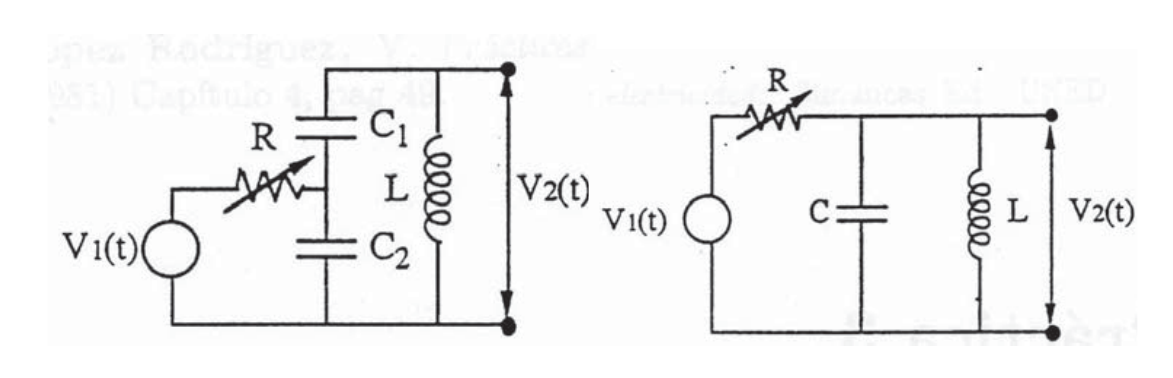
\includegraphics[width=0.65\linewidth]{fourier/rlc_circuito.png}
    \caption{Esquema del circuito RLC paralelo}
    \label{fig:enter-label}
\end{figure}

El circuito real con el que contamos en el laboratorio es es de la izquierda, mientras que el circuito de la derecha es el circuito equivalente aproximado teniendo en cuenta la composición de $C_1$ y $C_2$ en serie:

\begin{equation}
    C = \frac{C_1C_2}{C_1+C_2}
    \label{capacitancia}
\end{equation}

En la siguiente figura podemos ver el circuito empleado con sus respectivos componentes, la resistencia (1), los condensadores (2), la bobina (3), la entrada (4) y la salida (5):

\begin{figure}[h!]
    \centering
    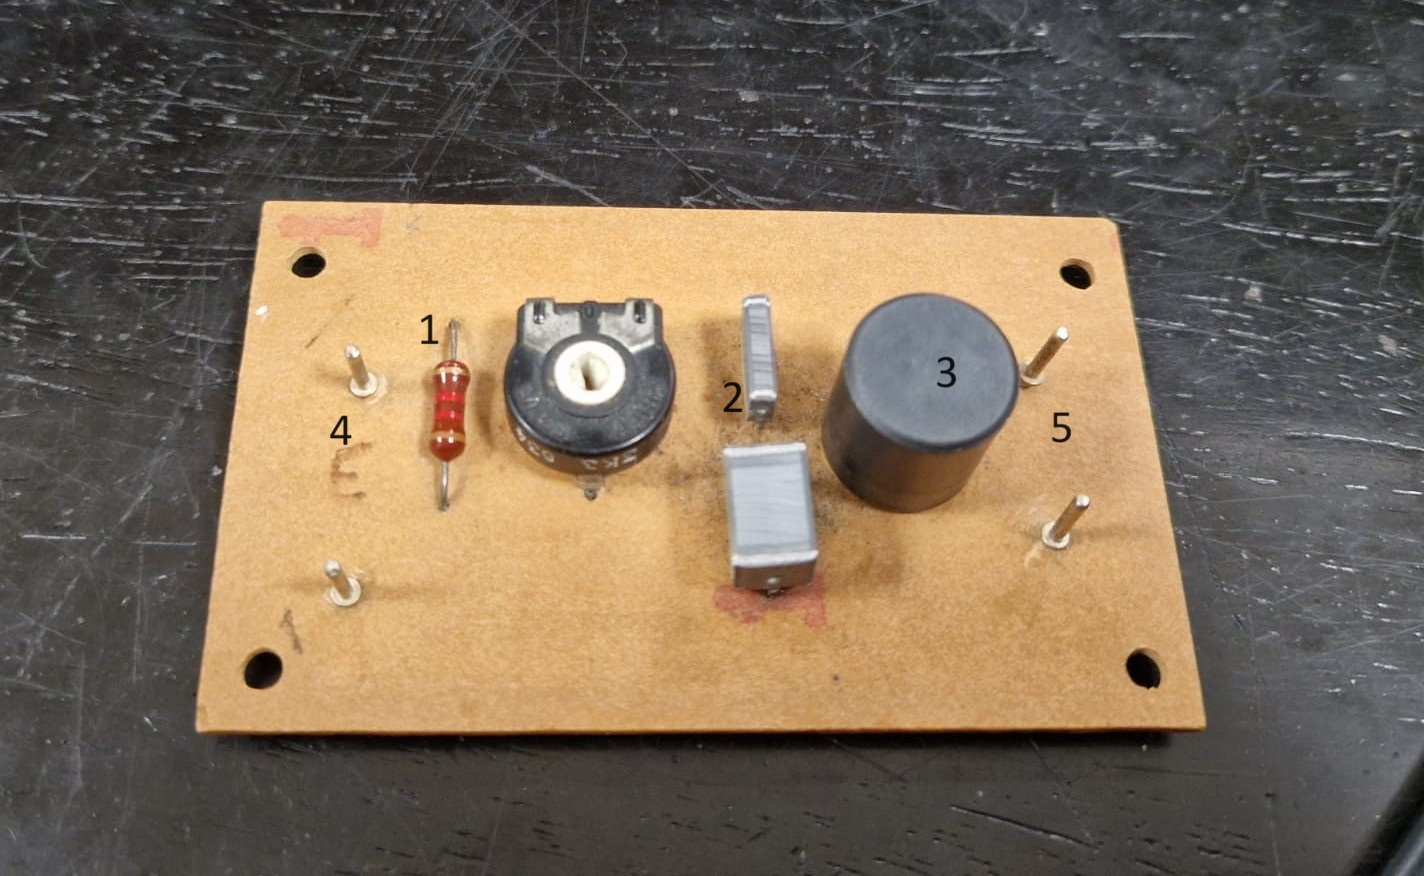
\includegraphics[width=0.65\linewidth]{fourier/rlc_paralelo_foto.jpg}
    \caption{Circuito empleado en el laboratorio}
    \label{fig:enter-label}
\end{figure}

\subsection{Metodología experimental}

Una vez detallado el montaje del circuito RLC resulta más sencillo ilustrar el procedimiento experimental, que se basará en transmitir una determinada señal por las conexiones de entrada y observar en el osciloscopio la respuesta del circuito.

\subsubsection{Determinación de los parámetros del circuito}

Antes de transmitir ninguna señal de corriente alterna concreta al circuito debemos determinar sus parámetros característicos: la frecuencia de resonancia $f_0$ y el ancho de banda. En este caso el factor de calidad $Q$ se podría obtener de forma trivial con un simple cálculo a partir de las magnitudes anteriores.

Para la determinación de la frecuencia de resonancia empleamos dos métodos, el método directo y el indirecto. Comenzaremos por el método indirecto, que se basa en la Ec.\ref{f0}, para la que necesitamos conocer los valores de la inductancia y la capacitancia de la bobina y los condensadores respectivamente. Estos valores dependen de los componentes empleados, cada uno tendrá su respectivo valor conocido de antemano. Este valor será empleado simplemente como referencia, por lo que no consideraremos una incertidumbre asociada.

Una vez obtenido el valor de $f_0$ de forma indirecta vamos a obtenerlo de forma directa, tomando este último valor como referencia. Para ello vamos a suministrar un voltaje de entrada sinusoidal y buscaremos la frecuencia de resonancia $f_0$, que será aquella que haga que el desfase entre la entrada y la salida sea nulo, además que la amplitud de la salida será máxima. La incertidumbre de esta frecuencia de resonancia vendrá dada por la precisión del generador de la corriente alterna.

Otra de las magnitudes a calcular es el ancho de banda del circuito, que vendrá dado por la Ec.\ref{band_w}. Para obtener el ancho de banda buscaremos con el generador de corriente alterna las frecuencias que generen un desfase de $\pm 45^{\circ}$, el ancho de banda será la longitud de este intervalo. A partir del ancho de banda y de la frecuencia de corte ya podremos calcular el factor de calidad $Q$ con la Ec.\ref{q_factor}.

\subsubsection{Análisis de Fourier}

Una vez conocidos los parámetros del circuito vamos a proceder al estudio de la respuesta del circuito a diferentes señales de corriente alterna, que introduciremos con nuestro generador AC. Para ello emplearemos, al igual que antes, el osciloscopio digital, que nos permite caracterizar la entrada y la salida del circuito de forma cuantitativa. En concreto caracterizaremos los armónicos no nulos de la señal de salida, que podrán ser los de la serie de senos o cosenos según la paridad de la señal, para analizar el comportamiento general que presenta el circuito frente a la señal introducida. 

Para buscar los armónicos introduciremos señales de entrada de la onda a estudiar de frecuencias $f_0/n$, frecuencias teóricas a las que se encuentran los armónicos. No obstante, estas frecuencias no son exactamente a las que se encuentran los armónicos, pero sirven de orientación para encontrarlos, cuando la amplitud de la salida sea máxima. Una vez encontremos estos máximos anotaremos el voltaje $V_{pp}=V_2$ de la salida, que se corresponden con el voltaje pico-pico de la señal de salida, que está directamente relacionado con los diferentes coeficientes de Fourier, como veremos más adelante.

Repetiremos este proceso para encontrar los 5 primeros armónicos de tres ondas diferentes: una onda cuadrada, una onda triangular y una delta de Dirac. Cabe destacar que la delta de Dirac será una aproximación creada en el laboratorio, para ello emplearemos el rectificador para truncar (eliminar la parte negativa) una señal triangular muy estrecha. La onda creada de esta forma se aproxima a una delta de Dirac, ya que es un pulso muy estrecho en comparación con su amplitud. Además de eso, para caracterizar la delta es necesario conocer la amplitud de su período, $T$, que mediremos con los cursores del osciloscopio.

Por último, cabe destacar que todas las medidas realizadas en el laboratorio fueron tomadas con el osciloscopio, incluidas las frecuencias de las señales de corriente alterna, pese a que estas fueron creadas con un generador AC que indicaba la propia frecuencia de la onda. Pese a esto, consideramos oportuno tomar como referencia el valor del osciloscopio, para que todas las medidas procedieran del mismo aparato. Cabe destacar que las diferencias entre las frecuencias del generador AC y las medidas por el osciloscopio son mínimas, no supondrán una gran fuente de error.

\newpage

\section{Resultados experimentales y tratamiento de datos}

\subsection{Parámetros característicos del circuito}

En primer lugar debemos caracterizar completamente el circuito con sus parámetros característicos, como ya hemos mencionado anteriormente. Como trabajamos con un circuito RLC las magnitudes que lo caracterizarán serán la resistencia $R$, la inductancia $L$ y la capacitancia $C$, que consideraremos que no tienen incertidumbres pues solo las necesitamos para buscar un valor de referencia para la frecuencia de resonancia.

En primer lugar, medimos el valor de la resistencia con el polímetro, obteniendo el siguiente resultado:

\begin{equation}
    R = 1190\; \Omega
\end{equation}

Por otro lado, el valor de la inductancia de la bobina viene anotado en el dispositivo. 

\begin{equation}
    L = 47 \;mH
\end{equation}

Por último, tenemos la capacitancia del circuito, que viene dada por la composición en serie de los dos condensadores, que podemos calcular a partir de la Ec.\ref{capacitancia}:

\begin{equation}
    C = 21 \; nF
\end{equation}

Teniendo en cuenta estos valores ya podemos caracterizar nuestro circuito. Comenzamos por la frecuencia de resonancia, que calcularemos a partir de la Ec.\ref{f0} para obtener su valor teórico. El valor obtenido es de:

\begin{equation}
    f_{0,T} = 5,11 \; kHz
\end{equation}

Tomando este valor como referencia vamos a buscar experimentalmente la frecuencia de resonancia, como explicamos en la metodología. El valor medido experimentalmente es de:

\begin{equation}
    f_0 = 4,92 \pm 0,05 \; kHZ
\end{equation}

Podemos ver que el valor medido experimentalmente no se corresponde con el teórico, pero difieren en apenas $0,2 \; kHz$. La incertidumbre del valor experimental de $f_0$ fue estimada en el laboratorio teniendo en cuenta las pequeñas oscilaciones de las medidas observadas.

A continuación obtuvimos el ancho de banda de la señal de salida, para ello medimos las frecuencias que hacían que el desfase fuera de $\pm 45^{\circ}$. Cabe destacar que el valor de $-45^{\circ}$ no aparece en el osciloscopio, se corresponde con una fase de $315^{\circ}$. Las frecuencias medidas son:

\begin{equation}
    f_{(\phi=45^{\circ})} = 5,02 \pm 0,05 \; kHz \quad f_{(\phi=-45^{\circ})} = 4,85 \pm 0,05 \; kHz
\end{equation}

Tomando estos resultados el ancho de banda de la salida es:

\begin{equation}
    B = 170 \; Hz \quad s(B) = \sqrt{2}\cdot s(f) = 71 \;Hz
\end{equation}

Podemos ver que la incertidumbre del ancho de banda es muy alta en comparación con el resultado. Esto es algo que se explica teniendo en cuenta que las incertidumbres de las frecuencias son relativamente altas, ya que trabajamos con frecuencias del orden de $kHz$, y al tomar un intervalo tan pequeño de frecuencias la incertidumbre se vuelve más significativa.

Por último, para caracterizar como de aguda es la resonancia podemos calcular el factor de calidad $Q$ a partir de la Ec.\ref{q_factor}. La incertidumbre se puede calcular por propagación a partir de la siguiente expresión:

\begin{equation}
    s(Q) = \sqrt{\frac{s(f_0)^2}{B^2} + \frac{f_0^2 s(B)^2}{B^4}}
\end{equation}

El valor obtenido para el factor de calidad es:

\begin{equation}
    Q = 29 \pm 12
\end{equation}

Podemos ver que, al igual que con $B$, la incertidumbre es enorme en comparación con el resultado, del mismo orden de magnitud. Esto se debe a las respectivas propagaciones que fuimos haciendo para llegar a la incertidumbre de este resultado, a pesar de que las incertidumbres de las frecuencias no son excesivas teniendo en cuenta los rangos en los que trabajamos.

\subsection{Onda cuadrada}

Una vez conocidos los parámetros característicos del circuito podemos pasar al estudio de las respuestas que este ofrece frente a diversas señales de entrada, empleando el análisis de Fourier.

Comenzaremos por una señal de entrada con forma de onda cuadrada, representada por la siguiente forma funcional:

\begin{equation}
    f(t) = \left\{ \begin{array}{ccc}
        -V & \text{si} & t\in \left[-\frac{T}{2},0)\right. \\ \\
        V & \text{si} & t\in \left.(0,\frac{T}{2}\right]
    \end{array} \right.
\end{equation}

Podemos ver que esta señal resulta ser una señal peródica impar, por lo que los coeficientes de Fourier a estudiar son los $b_n$, los coeficientes correspondientes a los cosenos se anulan. En la siguiente figura podemos apreciar una señal cuadrada en el osciloscopio así como la respuesta del circuito:

\begin{figure}[h!]
    \centering
    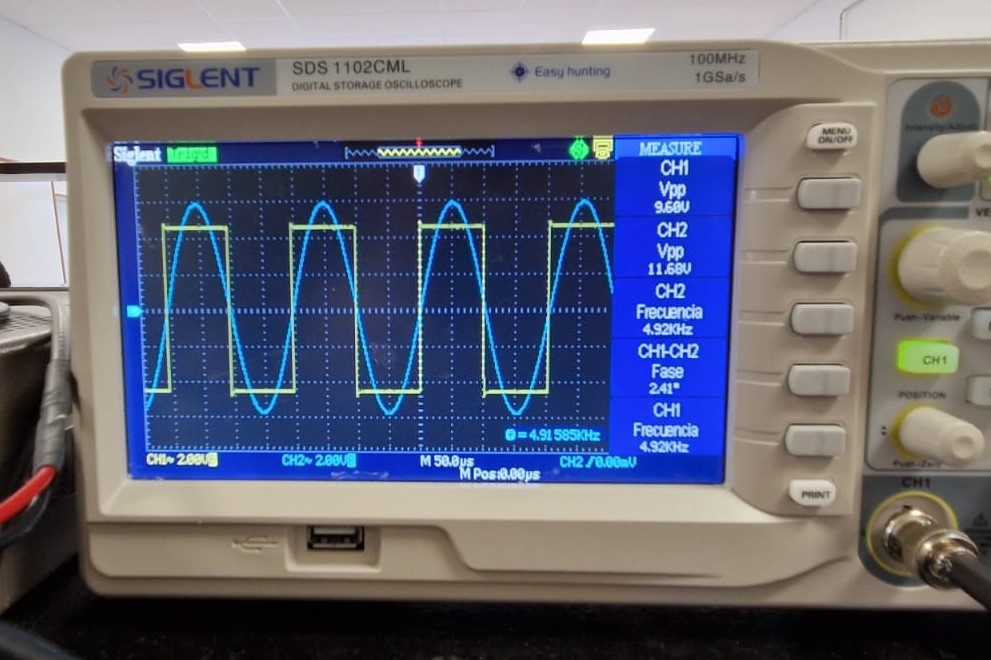
\includegraphics[width=0.6\linewidth]{fourier/onda cuadrada/cuadrada1.jpg}
    \caption{Señal de entrada cuadrada y respuesta del circuito}
    \label{arm1_c}
\end{figure}

Si realizamos el desarrollo en serie de Fourier de esta señal los $b_n$ obtenidos son:

\begin{equation}
    \begin{gathered}
        b_n = \frac{2}{T} \left[ \int_{-\frac{T}{2}}^0 -V\sin (n\omega t) \dd t + \int_0^{\frac{T}{2}} V\sin (n\omega t)\right] = \frac{4V}{n\omega T} \left[1 - \cos \left(\frac{n\omega T}{2}\right)\right] = \\
        = \frac{2V}{n\pi} (1-\cos n\pi) = \frac{2V}{n\pi} (1-(-1)^n)
    \end{gathered}
\end{equation}

A la vista de la última expresión podemos ver que los armónicos pares se anulan, solo existe solución no nula si $n=1,3,5,...$ Si hacemos el cambio de índice $n=2k-1$ con $k=1,2,3,...$ podemos escribir la señal cuadrada de entrada en su representación de serie de Fourier:

\begin{equation}
    f(t) = \sum_{k=1}^{\infty} \frac{4V}{(2k-1)\pi} \sin [(2k-1)\omega t]
\end{equation}

A partir de esta expresión podemos conocer el valor de los diferentes armónicos de la onda de entrada, conociendo el voltaje $V$, que no es más que la amplitud de la onda de entrada. Con el osciloscopio medimos voltajes pico-pico, desde el punto de mayor amplitud al de menor, por lo que para nuestra onda cuadrada el valor de $V$ es simplemente la mitad de los voltajes medidos con el osciloscopio para la señal de entrada:

\begin{equation}
    V = \frac{V_{pp}}{2} \quad s(V) = \frac{s(V_{pp})}{2}
\end{equation}

Durante las diferentes medidas realizadas con la onda cuadrada el voltaje de entrada $V_{pp}$ se mantuvo constante, con un valor de $9,60 \pm 0,40 \;V$, por tanto el voltaje $V$ de la onda de entrada es:

\begin{equation}
    V = 4,80 \pm 0,20 \;V
\end{equation}

Conociendo este valor ya tenemos totalmente definidos los valores teóricos de los diferentes armónicos de la señal, que mediremos en el laboratorio con el osciloscopio. Los valores teóricos de los armónicos no nulos, según el desarrollo de Fourier anterior, siguen la siguiente expresión:

\begin{equation}
    b_k = \frac{4}{(2k-1)\pi} (V \pm s(V)) \quad k=1,2,3,...
\end{equation}

Si sustituimos el valor de $V$ medido con el osciloscopio podemos obtener el resultado numérico del valor teórico de los coeficientes de Fourier no nulos:

\begin{table}[h!]
\centering
\begin{tabular}{|c|c|c|}
\hline
n & $b_n \;(V)$ & $s(b_n) \;(V)$ \\ \hline
1 & $6,11$ & $0,25$ \\ \hline
3 & $2,037$ & $0,085$ \\ \hline
5 & $1,222$ & $0,051$ \\ \hline
\end{tabular}
\caption{Armónicos teóricos de la onda cuadrada y sus incertidumbres}
\label{tab:my-table}
\end{table}

\newpage

Una vez calculados los valores teóricos vamos a compararlos con los medidos experimentalmente con el osciloscopio. Medimos solo los cinco primeros pues el resultado del armónico decrece de la forma $1/n$, siendo cada vez los voltajes de salida más pequeño, tendiendo a cero. Para medirlos, como ya explicamos antes, fijamos la frecuencia de la onda de entrada en los valores $f_0/n$ y medimos los voltajes de salida del circuito. Estos voltajes se deberían corresponder con los diferentes armónicos de la señal de entrada. Los resultados obtenidos para los armónicos no nulos fueron:

\begin{table}[h!]
\centering
\begin{tabular}{|c|c|c|c|}
\hline
n & $f \pm 0,05 \; (kHz)$ & $b_n \;(V)$ & $s(b_n) \; (V)$ \\ \hline
1 & $4,92$ & $5,9$& $0,2$   \\ \hline
3 & $1,63$ &  $1,8$& $0,1$   \\ \hline
5 & $0,98$ &  $1,19$& $0,05$  \\ \hline
\end{tabular}
\caption{Armónicos experimentales de la onda cuadrada}
\label{tab:my-table}
\end{table}

En las siguientes imágenes podemos ver las respuestas del circuito al tercer y al quinto armónico, el primer armónico se corresponde con la Fig.\ref{arm1_c}:

\begin{figure}[h!]
    \centering
    \begin{subfigure}{0.49\textwidth}
        \centering
        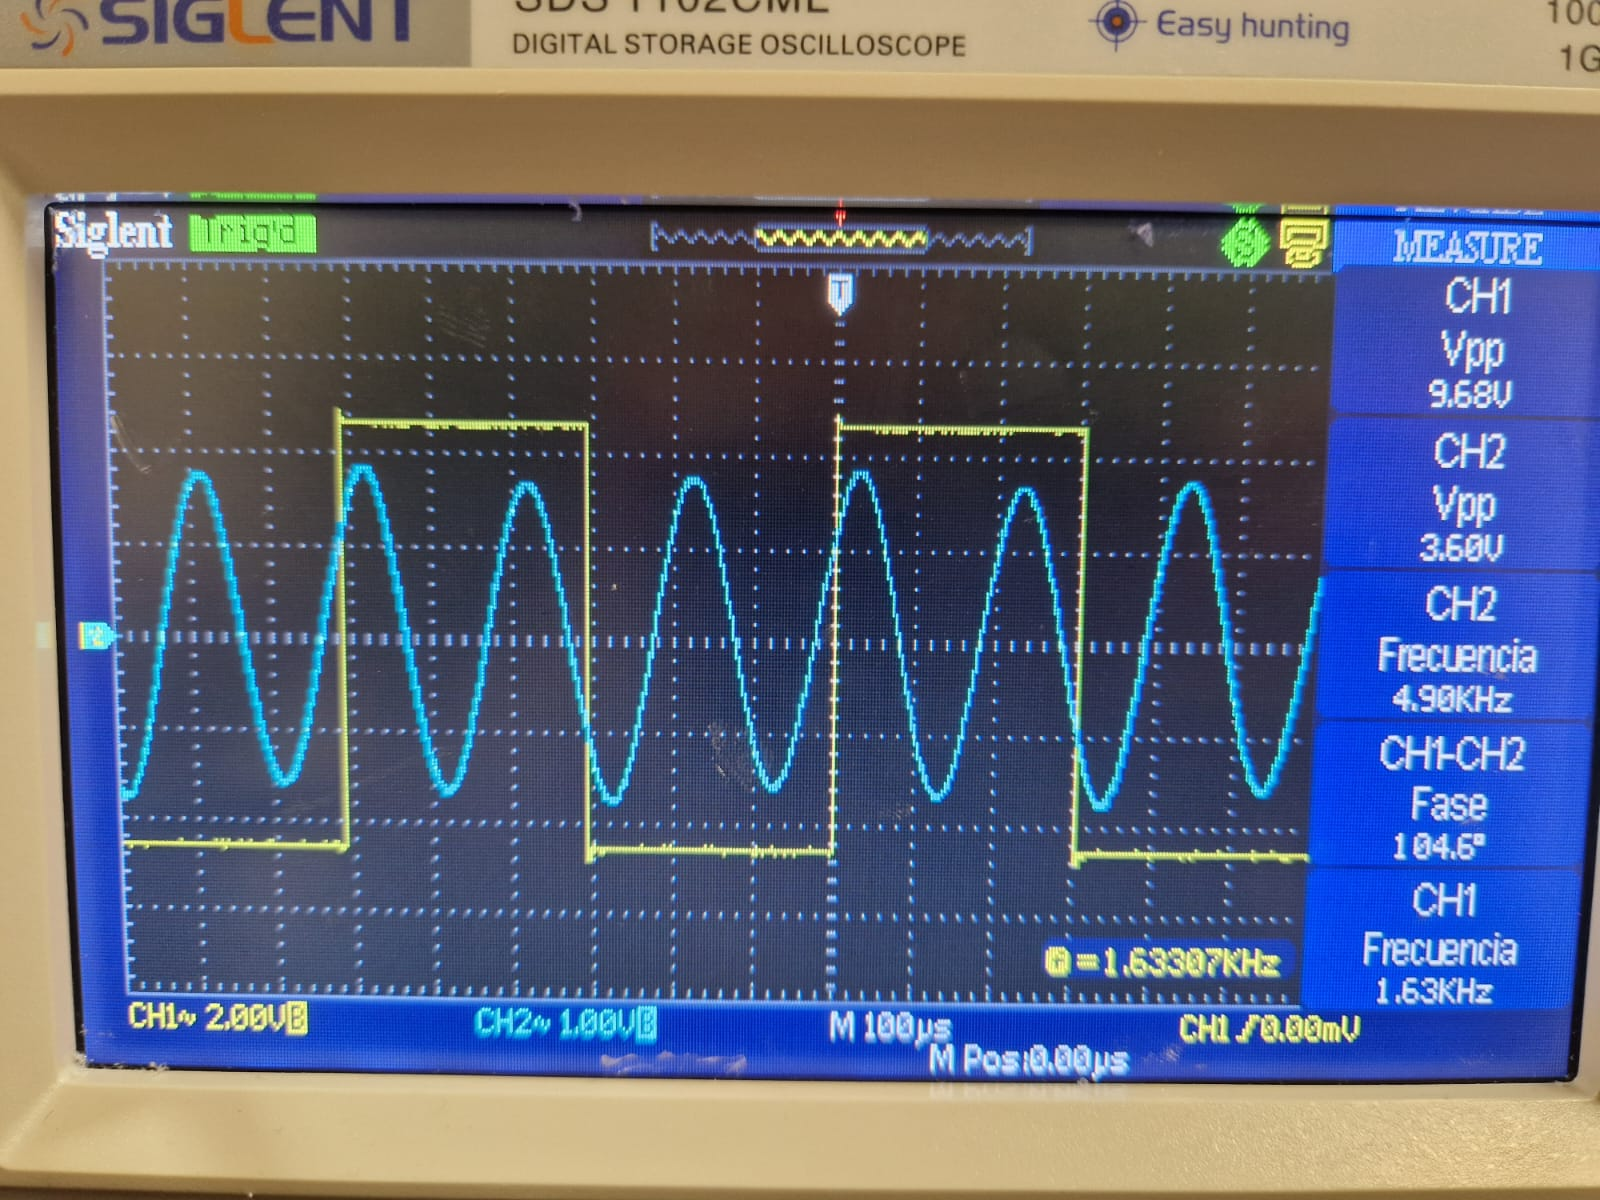
\includegraphics[width=0.75\linewidth]{fourier/onda cuadrada/cuadrada3.jpg}
        \subcaption{2º armónico}
    \end{subfigure}
    \begin{subfigure}{0.49\textwidth}
        \centering
        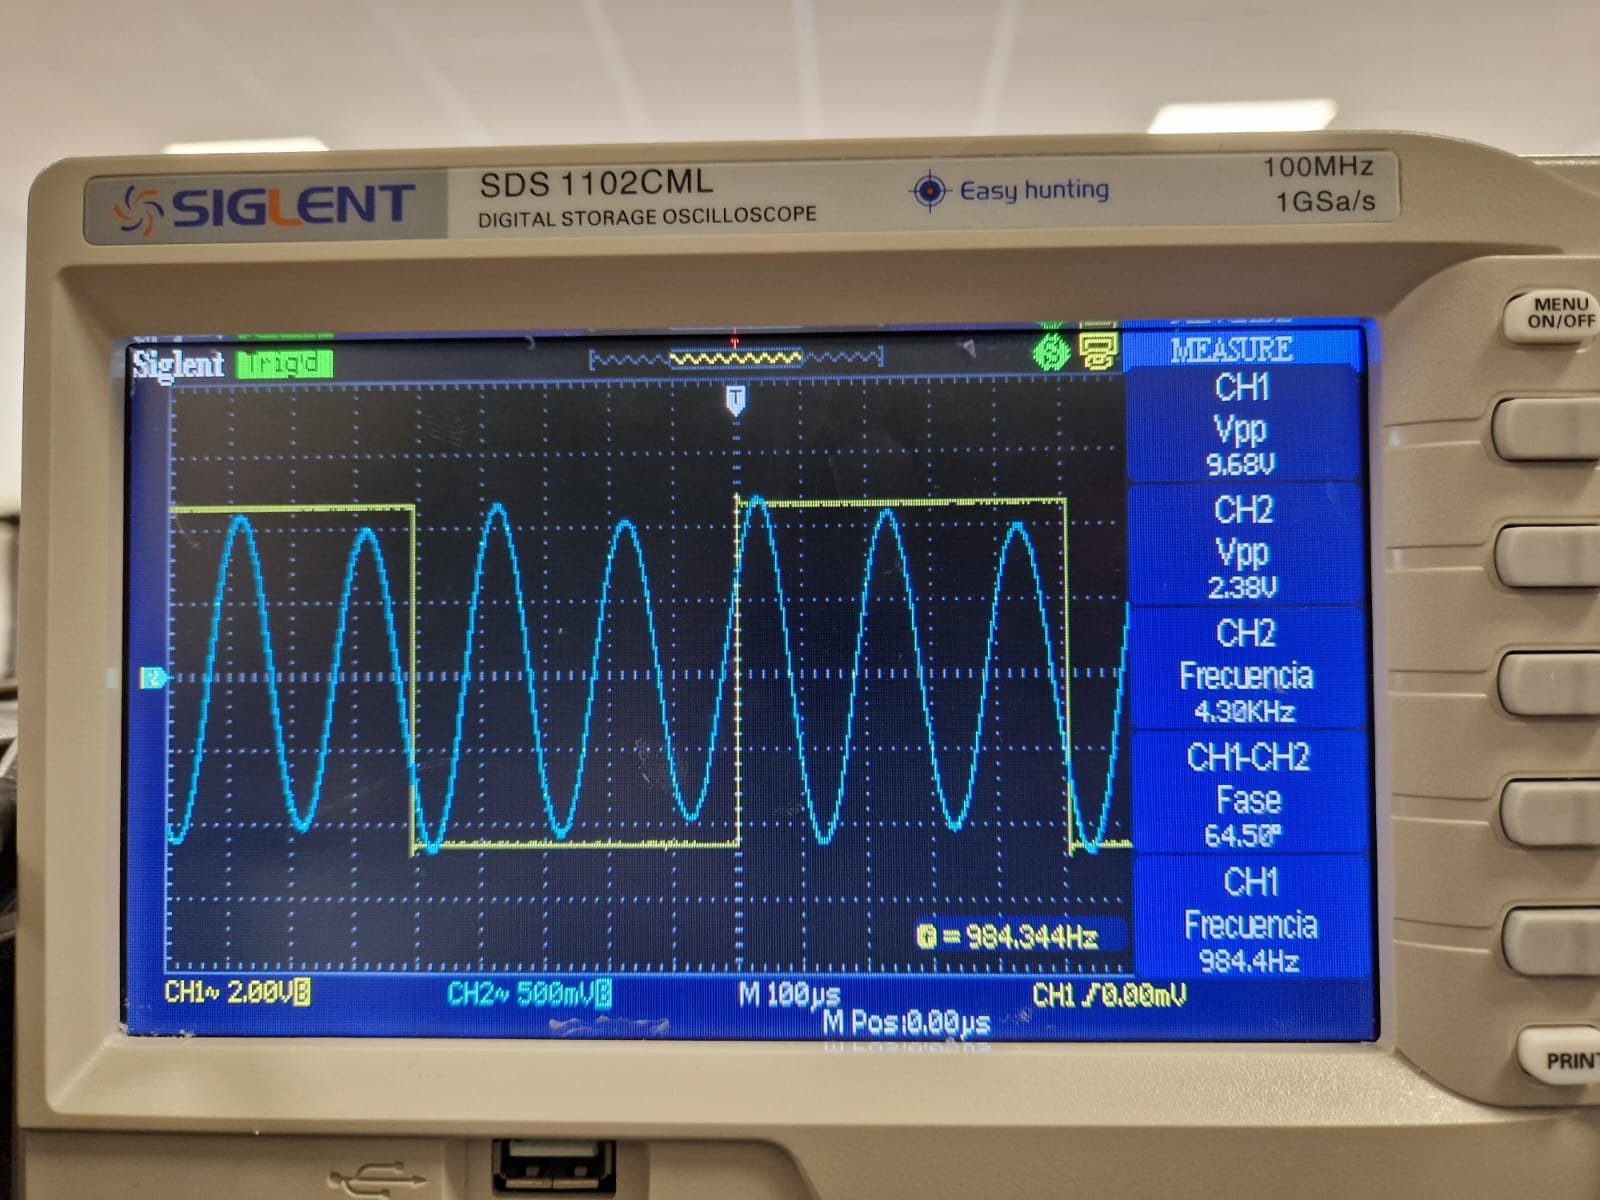
\includegraphics[width=0.75\linewidth]{fourier/onda cuadrada/cuadrada2.jpg}
        \subcaption{3º armónico}
    \end{subfigure}
    \caption{Respuestas del circuito a los diferentes armónicos}
    \label{fig:enter-label}
\end{figure}

\begin{figure}[h!]
    \centering
    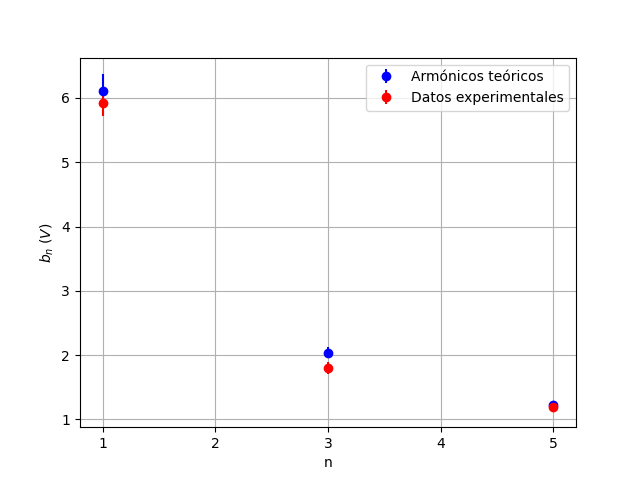
\includegraphics[width=0.515\linewidth]{fourier/arm_cuadrada.png}
    \caption{Armónicos de la onda cuadrada}
    \label{fig:enter-label}
\end{figure}


En la última figura podemos ver una representación gráfica de los tres armónicos no nulos con sus respectivas barras de incertidumbre, comparando los valores teóricos con los medidos experimentalmente. Aquí se puede ver perfectamente la tendencia de los armónicos, estando los valores experimentales siempre por debajo de los valores teóricos que le correspondían.

\subsection{Onda triangular}

El procedimiento a realizar con la onda triangular es idéntico, vamos a realizar el análisis de Fourier de esta señal para calcular sus armónicos, que compararemos con los experimentales. La función que describe la señal cuadrada es una función lineal en $t$ y definida a trozos que tiene la siguiente expresión:

\begin{equation}
    f(t) = \left\{ \begin{array}{ccc}
        V + \frac{4V}{T} t  & \text{si} & t\in \left[-\frac{T}{2},0)\right. \\ \\
        V -\frac{4V}{T} t & \text{si} & t\in \left.(0,\frac{T}{2}\right]
    \end{array} \right.
\end{equation}

\begin{figure}[h!]
    \centering
    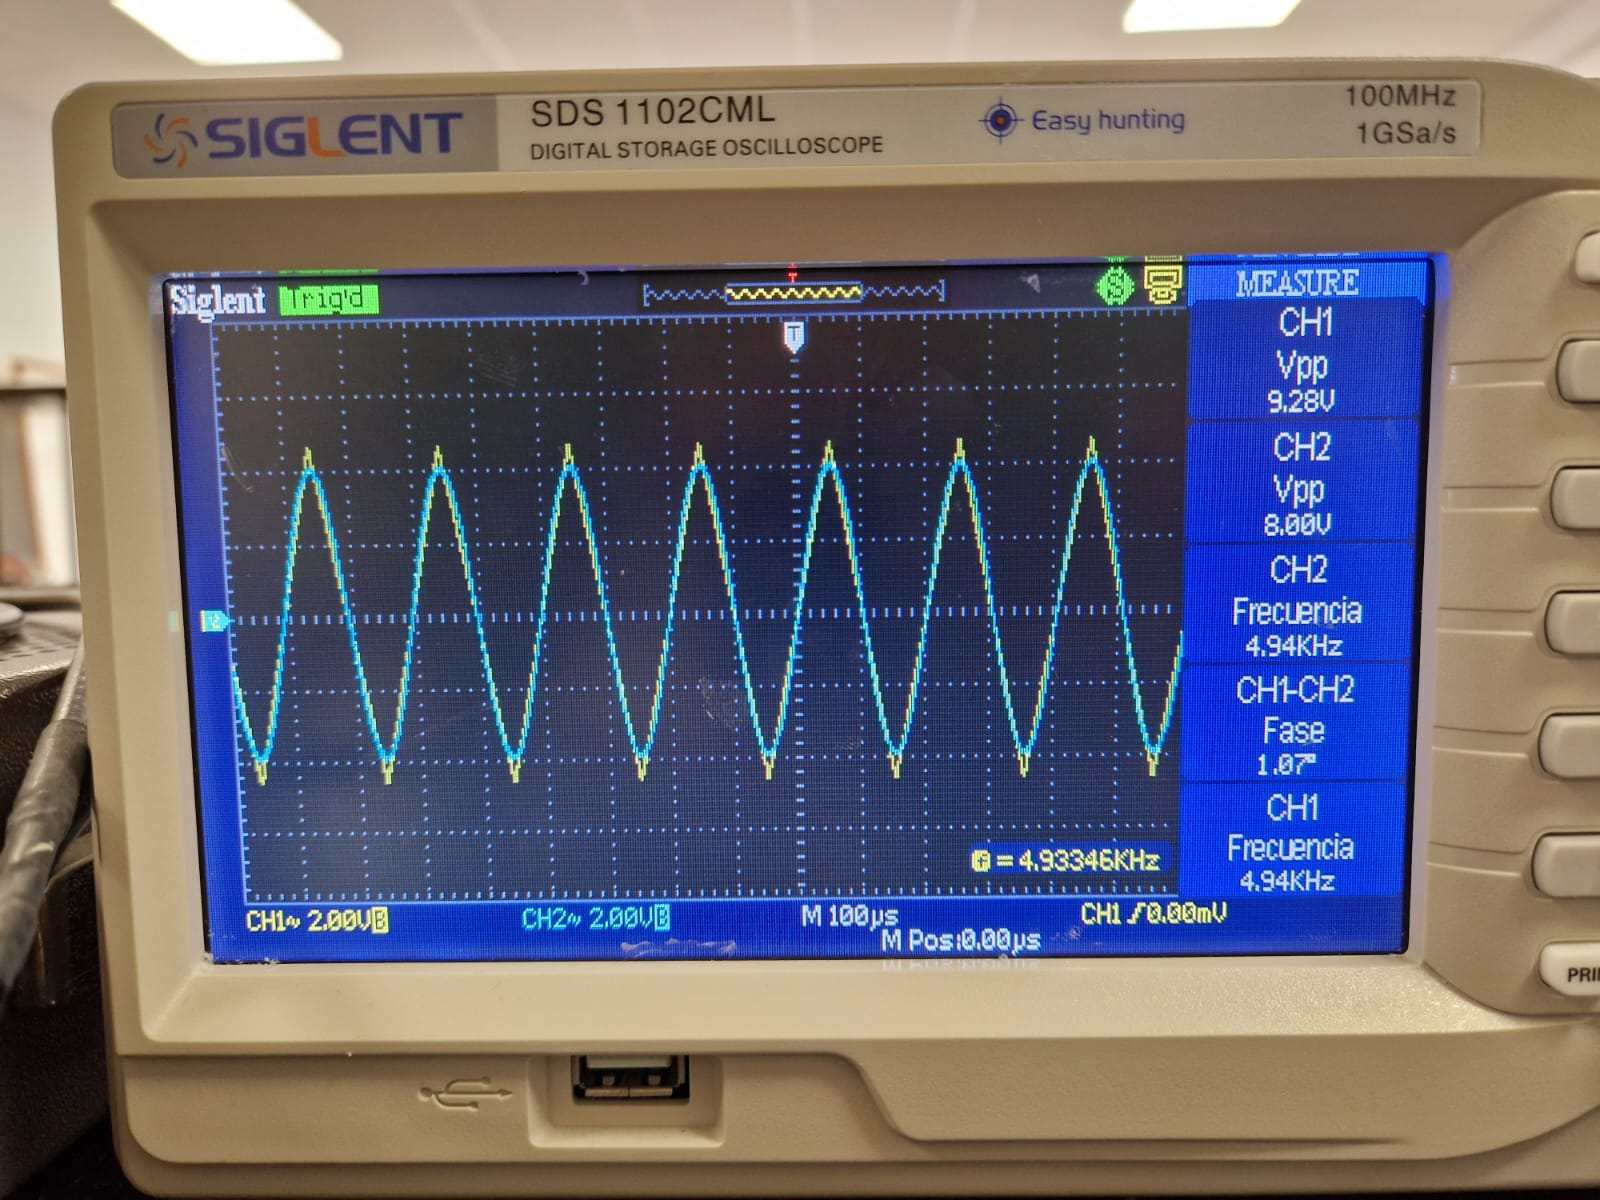
\includegraphics[width=0.5\linewidth]{fourier/onda triangular/triangular1.jpg}
    \caption{Señal de entrada triangular y respuesta del circuito}
    \label{arm_1t}
\end{figure}

Una vez tenemos la forma funcional de la onda podemos calcular sus coeficientes de Fourier, de igual forma que con la onda cuadrada. En este caso la onda triangular es una función par, por lo que los coeficientes $b_n$ que acompañan a los senos se anulan, solo tenemos los $a_n$, que tienen la siguiente expresión:

\begin{equation}
    \begin{gathered}
        a_0 = \frac{4}{T} \int_0^{T/2} \left( V-\frac{4V}{T} t \right) \dd t = 0 \\
        a_n = \frac{4}{T} \int_0^{T/2} \left( V-\frac{4V}{T} t \right) \cos (n\omega t) \dd t = \frac{4V}{\pi^2 n^2} (1-\cos n\pi)
    \end{gathered}
\end{equation}


Como $\cos(n\pi)=(-1)^n$ podemos ver que los coeficientes pares se anulan, al igual que con la onda cuadrada. Además de eso empleamos que el integrando de la integral de los $a_n$ es una función para para agrupar las dos integrales. Si hacemos el cambio de índice $n=2k-1$ para quedarnos solo con los armónicos impares podemos expresar la serie de Fourier de una forma sencilla:

\begin{equation}
    f(t) = \sum_{k=1}^{\infty} \frac{8V}{\pi^2(2k-1)^2} \cos [(2k-1)\omega t]
\end{equation}

Donde $V$ es el voltaje máximo de la onda triangular de entrada que ,al igual que antes, se corresponde con la mitad del voltaje pico-pico medido en el osciloscopio. Por tanto, los coeficientes de Fourier teóricos de la onda triangular siguen la siguiente expresión:

\begin{equation}
    a_k = \frac{8}{\pi^2 (2k-1)^2} (V\pm s(V)) \quad k=1,2,3,...
\end{equation}

Sustituyendo el valor del voltaje máximo de la onda de entrada, que en este caso es $V = 4,6\pm 0,2 \; V$, la mitad del voltaje pico-pico, podemos calcular los valores teóricos de los coeficientes con sus respectivas incertidumbres:

\begin{table}[h!]
\centering
\begin{tabular}{|c|c|c|}
\hline
n & $b_n \;(V)$ & $s(b_n) \;(V)$ \\ \hline
1 & $3,73$ & $0,16$ \\ \hline
3 & $0,414$ & $0,018$ \\ \hline
5 & $0,1491$ & $0,0065$ \\ \hline
\end{tabular}
\caption{Armónicos teóricos de la onda triangular y sus incertidumbres}
\label{tab:my-table}
\end{table}

Una vez calculados los valores teóricos vamos a compararlos con los medidos con el osciloscopio. Al igual que antes, mediremos los cinco primeros armónicos, ya que decaen de la forma $1/n^2$ y tienden a cero muy rápido. Para medirlos, al igual que antes, fijamos frecuencias $f_0/n$ y medimos los voltajes de salida del circuito. Los resultados obtenidos fueron:

\begin{table}[h!]
\centering
\begin{tabular}{|c|c|c|c|}
\hline
n & $f \pm 0,05 \; (kHz)$ & $b_n \;(V)$ & $s(b_n) \; (V)$ \\ \hline
1 & $4,92$ & $4,0$& $0,2$   \\ \hline
3 & $1,64$ &  $0,39$& $0,02$   \\ \hline
5 & $0,98$ &  $0,166$& $0,005$  \\ \hline
\end{tabular}
\caption{Armónicos experimentales de la onda triangular}
\label{tab:my-table}
\end{table}

\begin{figure}[h!]
    \centering
    \begin{subfigure}{0.49\textwidth}
        \centering
        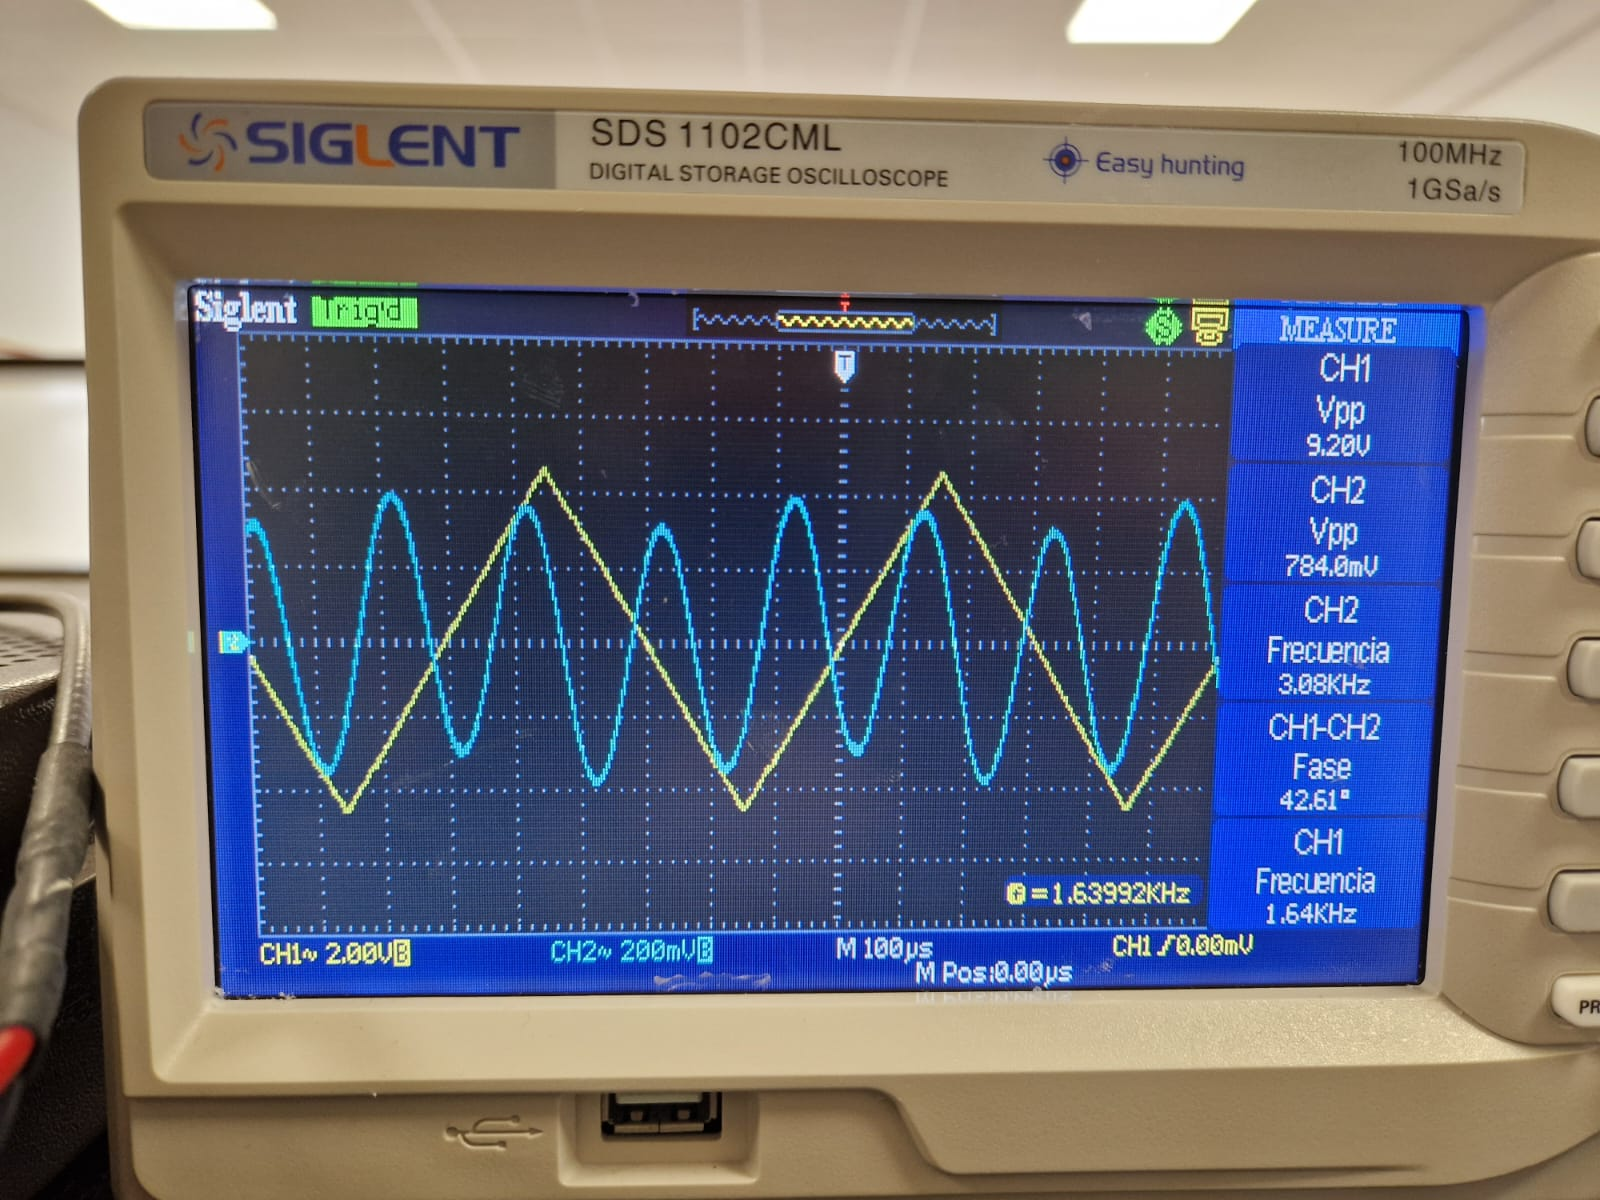
\includegraphics[width=0.8\linewidth]{fourier/onda triangular/triangular2.jpg}
        \subcaption{2º armónico}
    \end{subfigure}
    \begin{subfigure}{0.49\textwidth}
        \centering
        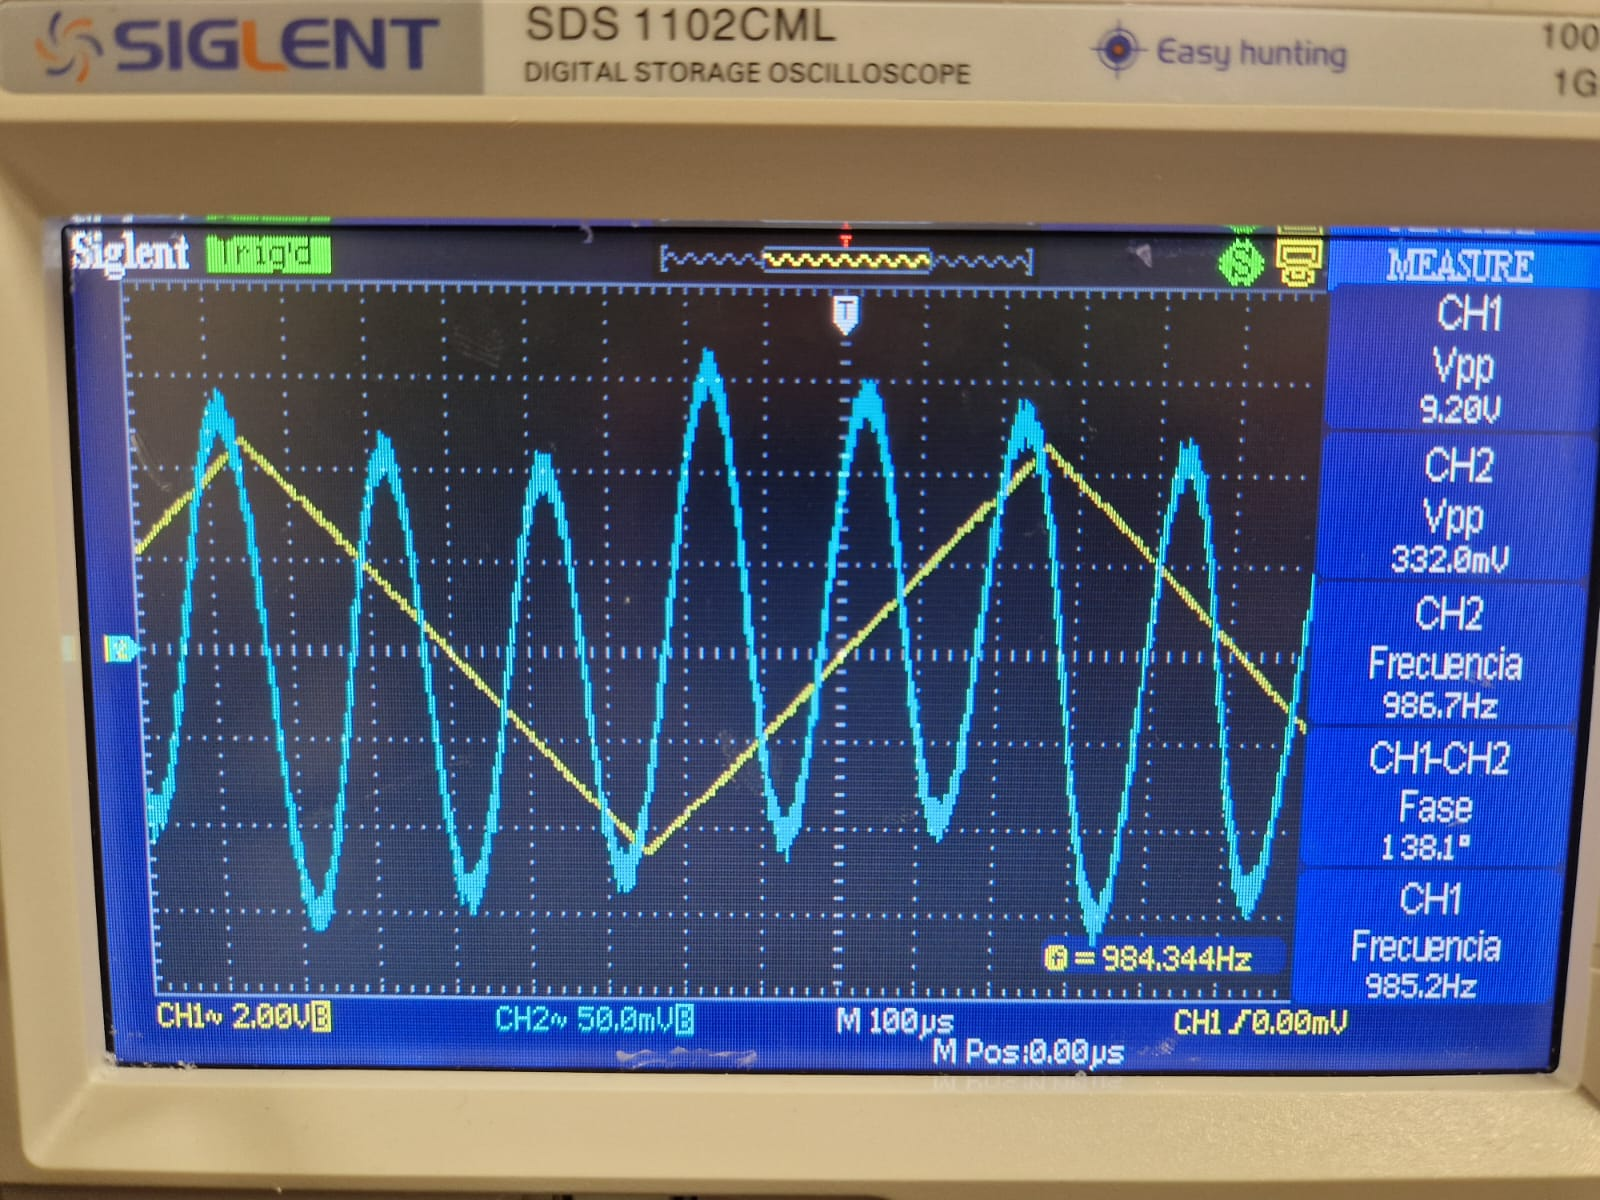
\includegraphics[width=0.8\linewidth]{fourier/onda triangular/triangular3.jpg}
        \subcaption{3º armónico}
    \end{subfigure}
    \caption{Respuestas del circuito a los diferentes armónicos}
    \label{fig:enter-label}
\end{figure}


En las imágenes anteriores podemos ver las respuestas del circuito al tercer y al quinto armónico, el primer armónico se corresponde con la Fig.\ref{arm_1t}.

En la siguiente figura podemos ver una representación gráfica de los tres armónicos no nulos, comparando los valores teóricos con los resultados experimentales:

\begin{figure}[h!]
    \centering
    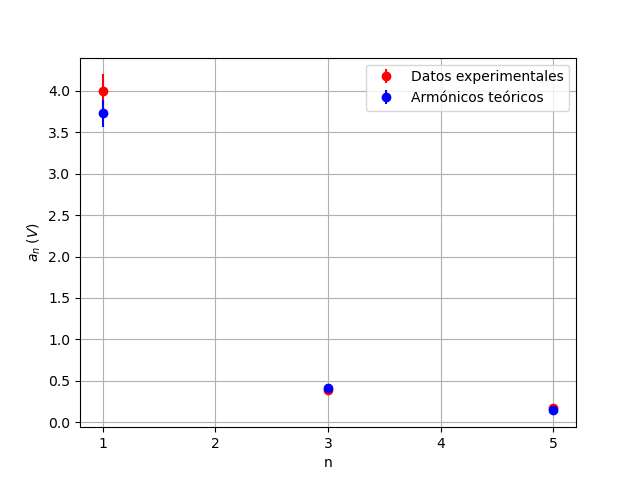
\includegraphics[width=0.6\linewidth]{fourier/arm_triangular.png}
    \caption{Armónicos de la onda triangular}
    \label{fig:enter-label}
\end{figure}

Podemos ver que los resultados experimentales se ajustan bastante bien a los valores teóricos, siendo el primer armónico el único que presenta cierta desviación.

\subsection{Delta de Dirac}

La última señal a analizar es un pulso con forma de delta de Dirac, ya que obtener una delta de Dirac en el laboratorio es algo imposible, por ser esta una función generalizada que no es continua. Para obtener un pulso similar a una delta vamos a emplear una señal triangular muy estrecha y aguda que se aproxime a la forma deseada. Además de eso, como ya hemos mencionado antes, contaremos con un rectificador para eliminar las contribuciones negativas de la onda. Para obtener una forma funcional para la señal vamos a caracterizar la entrada midiendo con el osciloscopio su altura, $V$, su anchura, $a$, y su período $T$. 

\begin{table}[h!]
\centering
\begin{tabular}{|c|c|}
\hline
$V\pm s(V)\; (V)$ & $1,820 \pm 0,004$\\ \hline
$a \pm s(a)\; (\mu s)$ &  $56 \pm 1$\\ \hline
$T \pm s(T)\; (\mu s)$ &  $612 \pm 6$\\ \hline
\end{tabular}
\caption{Magnitudes características del pulso}
\label{tab:my-table}
\end{table}

En la siguiente figura podemos ver el proceso de caracterización del pulso llevado a cabo en el laboratorio con el osciloscopio:

\newpage

\begin{figure}[h!]
    \centering
    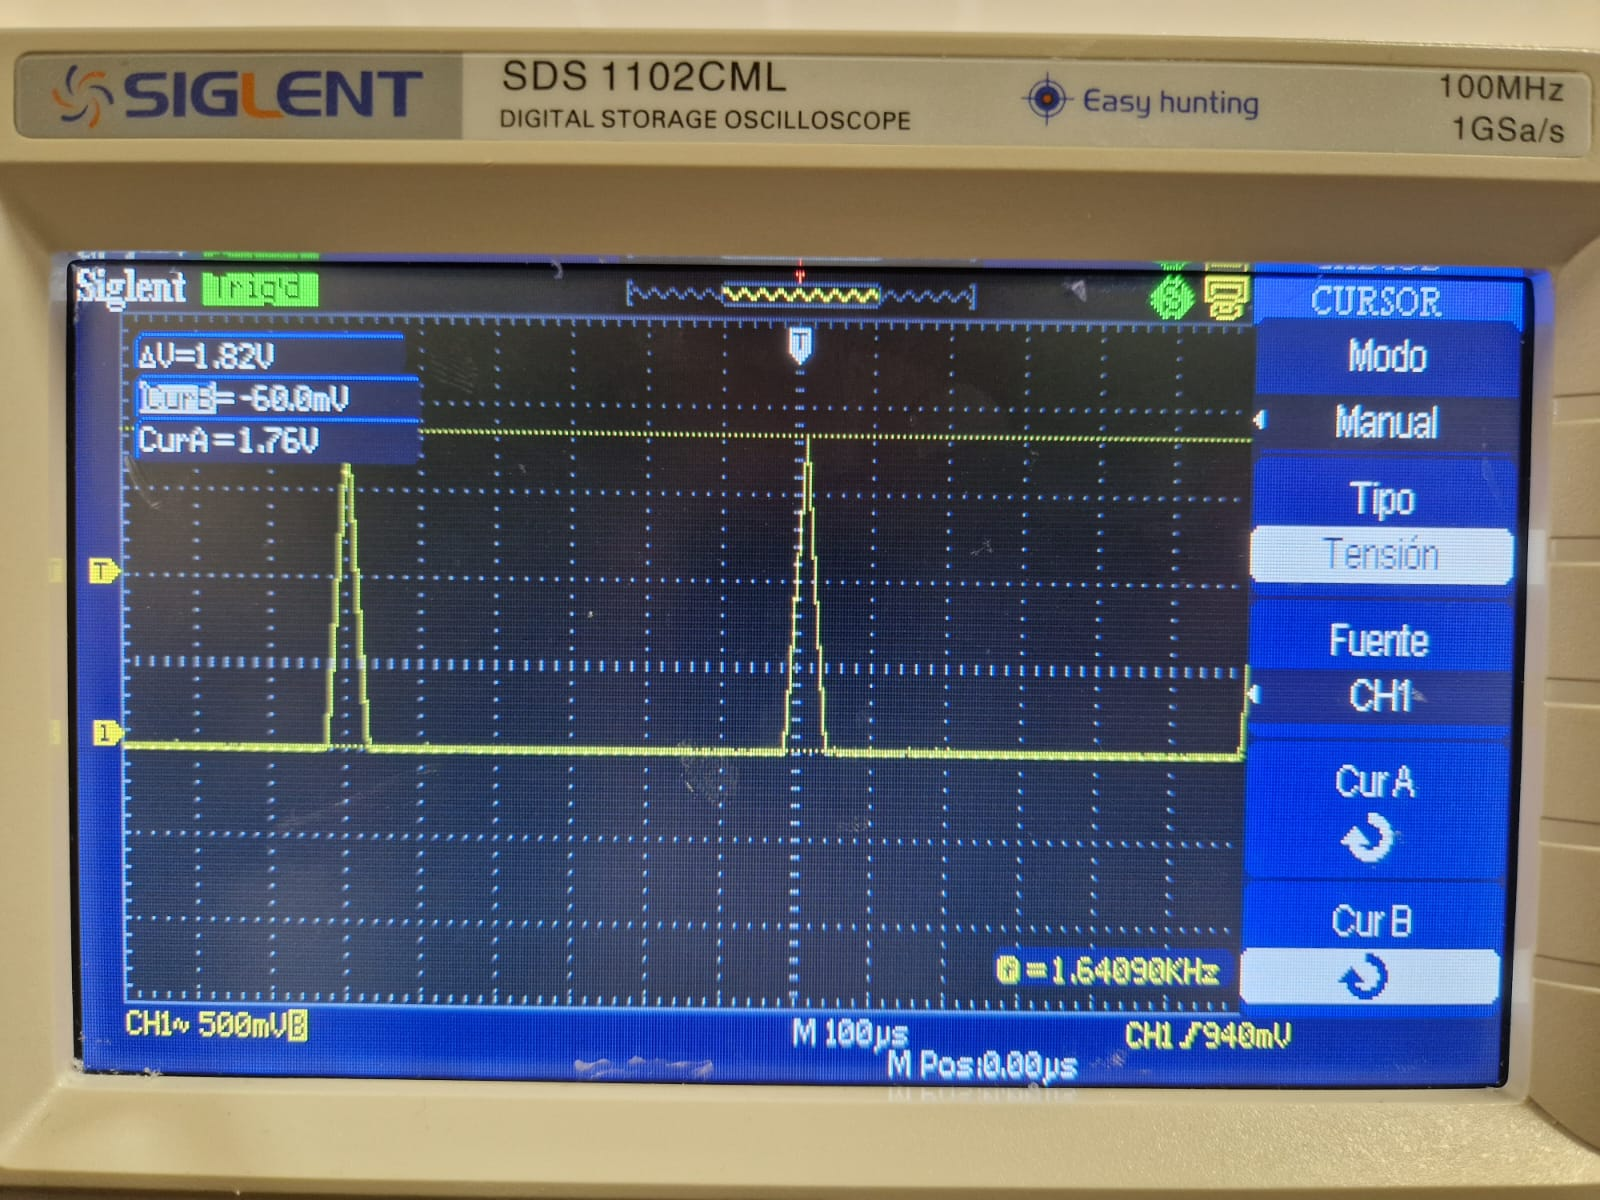
\includegraphics[width=0.5\linewidth]{fourier/delta_dirac/caracterizacion_delta.jpg}
    \caption{Caracterización de la delta de Dirac}
    \label{fig:enter-label}
\end{figure}

Con las tres magnitudes características de esta onda podemos obtener la siguiente forma funcional para la señal:

\begin{equation}
    f(t) = \left\{ \begin{array}{ccc}
        0 & si & t\in \left[-\frac{-T}{2},-a\right) \\ \\
        V + \frac{V}{a}t & si & t\in[-a,0) \\ \\
        V - \frac{V}{a}t & si & t\in[0,a) \\ \\
        0 & si & t\in \left(a,\frac{T}{2}\right]
    \end{array} \right.
\end{equation}

Al igual que la señal triangular, el pulso es una función par, los únicos términos no nulos son los $a_n$. Las expresiones para los coeficientes de Fourier obtenidas a partir de la forma funcional son:

\begin{equation}
    \begin{gathered}
        a_0 = \frac{4}{T} \int_0^a \left( V - \frac{V}{a}t\right) \dd t\ = \frac{2aV}{T} \\
        a_n =  \frac{4}{T} \int_0^a \left( V - \frac{V}{a}t\right) \cos (n\omega t) \dd t = \frac{4V}{\tan^2 \omega^2} [1- \cos (n\omega t)] = \frac{2VT}{\tan^2\pi^2} \sin^2 \frac{n\pi a}{T}
    \end{gathered}
    \label{an delta}
\end{equation}

Donde empleamos que el integrando es una función par para realizar solo una integral, además de las relaciones $T=2\pi/\omega$ y $1-\cos x = 2\sin^2 (x/2)$. Por tanto, el desarrollo de Fourier de la señal toma la siguiente expresión:

\begin{equation}
    f(t) = \frac{2aV}{T} + \sum_{n=1}^{\infty} \frac{2VT}{\tan^2\pi^2} \sin^2 \left(\frac{n\pi a}{T}\right) \cos \left(\frac{2\pi n a}{T} \right)
\end{equation}

Al igual que con las señales anteriores, si sustituimos $V$ por el valor del voltaje de la señal de entrada podemos obtener los valores teóricos de los coeficientes de Fourier empleando la Ec.\ref{an delta}. Los resultados obtenidos para un voltaje de entrada de $V=1,8 \pm 0,2 \;V$ son:

\newpage

\begin{table}[h!]
\centering
\begin{tabular}{|c|c|c|}
\hline
n & $V\;(V)$ & $s(V)\;(V)$ \\ \hline
1 & $0,171$ & $0,076$ \\ \hline
2 & $0,167$ & $0,071$ \\ \hline
3 & $0,162$ & $0,064$ \\ \hline
4 & $0,154$ & $0,054$ \\ \hline
5 & $0,144$ & $0,042$ \\ \hline
\end{tabular}
\caption{Coeficientes de Fourier teóricos para el pulso}
\label{tab:my-table}
\end{table}

La incertidumbre de los coeficientes tiene una expresión más complicada que la de las dos señales anteriores, ya que los $a_n$ ahora dependen también de las magnitudes características de la onda, ya no son una función lineal en el voltaje. Por tanto, la incertidumbre de estos coeficientes se puede calcular por propagación a partir de la siguiente expresión:

\begin{equation}
    \begin{gathered}
        \sqrt{A^2 s(V)^2 + B^2 s(a)^2 + C^2 s(T)^2} \\
        A = \pdv{a_n}{V} = \frac{2T}{an^2\pi^2} \sin^2 \left(\frac{n\pi a}{T} \right) \\
        B = \pdv{a_n}{a} = \frac{2V}{n \pi a} \left( 2 \sin \left(\frac{2n\pi a}{T} \right) - \frac{T}{n \pi a} \sin^2 \left( \frac{n\pi a}{T} \right) \right) \\
        C = \pdv{a_n}{T} = \frac{2V}{n\pi} \left( \frac{\sin^2 \left(\frac{n\pi a}{T}\right)}{n\pi a} - \frac{\sin \left(\frac{2n\pi a}{T}\right)}{T} \right)
    \end{gathered}
\end{equation}

Una vez tenemos los armónicos teóricos del pulso vamos a compararlos con los valores medidos experimentalmente. El procedimiento experimental es idéntico al seguido con las señales anteriores, fijamos las frecuencias $f_0/n$ y medimos $V_{pp}$ de la señal de salida. De esta forma estamos midiendo los voltajes pico-pico por lo que para tener el resultado de los armónicos tenemos que dividir estos valores entre 2, $a_n = V_{pp}/2$. Los resultados experimentales obtenidos son:

\begin{table}[h!]
\centering
\begin{tabular}{|c|c|c|c|}
\hline
n & $f \pm 0,05 \;(kHz)$ & $a_n\;(V)$ & $s(a_n)\;(V)$ \\ \hline
1 & $4,99$ & $0,216$ & $0,010$\\ \hline
2 & $2,52$ & $0,210$ & $0,010$\\ \hline
3 & $1,66$ & $0,206$ & $0,010$\\ \hline
4 & $1,25$ & $0,203$ & $0,010$\\ \hline
5 & $1,00$ & $0,199$ & $0,010$\\ \hline
\end{tabular}
\caption{Coeficientes de Fourier experimentales para el pulso}
\label{tab:my-table}
\end{table}

En este caso hemos considerado una incertidumbre con dos cifras significativas en lugar de una, como veníamos haciendo anteriormente por la resolución del osciloscopio. No obstante, consideramos que era necesario dar los resultados con tres decimales para poder apreciar realmente la tendencia que siguen, por lo que decidimos expresar la incertidumbre con dos cifras significativas.

En la siguiente figura podemos ver los tres primeros armónicos de nuestro pulso y la respuesta que da el circuito:

\newpage

\begin{figure}[h!]
    \centering
    \begin{subfigure}{0.45\textwidth}
        \centering
        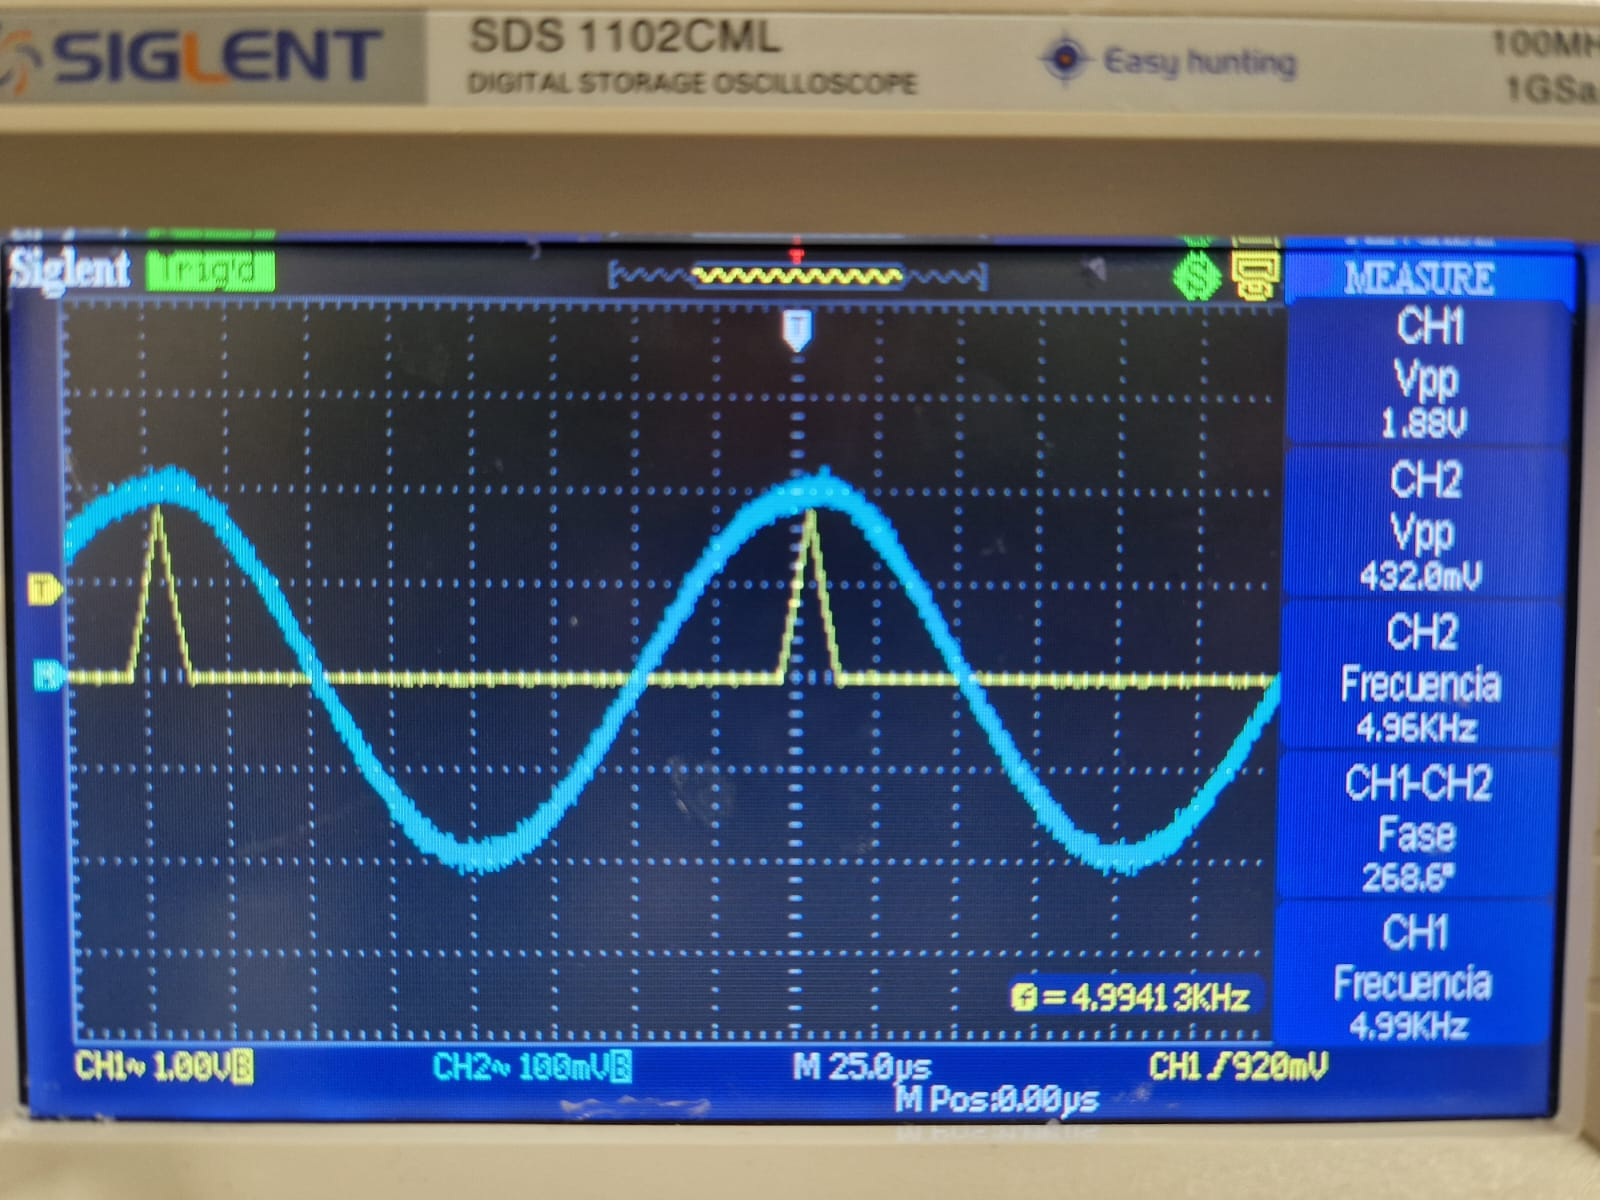
\includegraphics[width=1.05\linewidth]{fourier/delta_dirac/delta1.jpg}
        \subcaption{$n=1$}
        \label{fig:subfig1}
    \end{subfigure}
    \hfill
    \begin{subfigure}{0.45\textwidth}
        \centering
        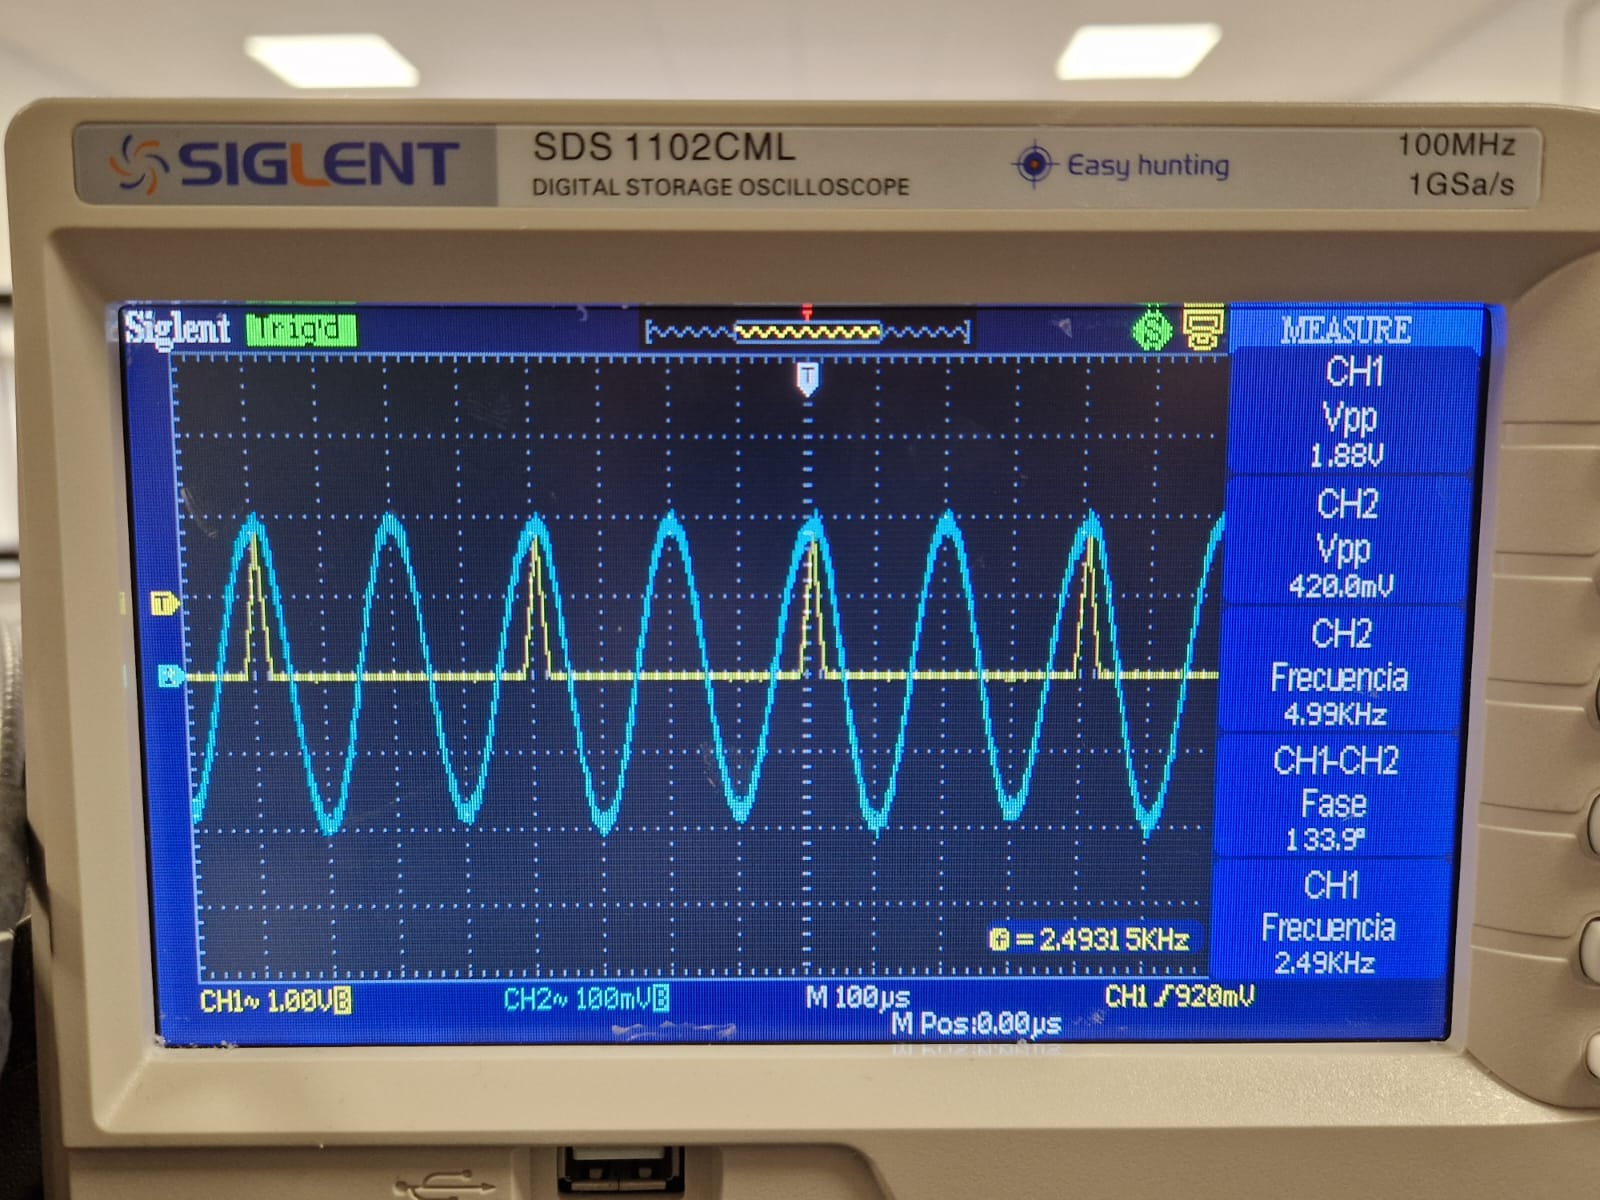
\includegraphics[width=1.05\linewidth]{fourier/delta_dirac/delta2.jpg}
        \subcaption{$n=2$}
        \label{fig:subfig2}
    \end{subfigure}
    \\
    \begin{subfigure}{0.45\textwidth}
        \centering
        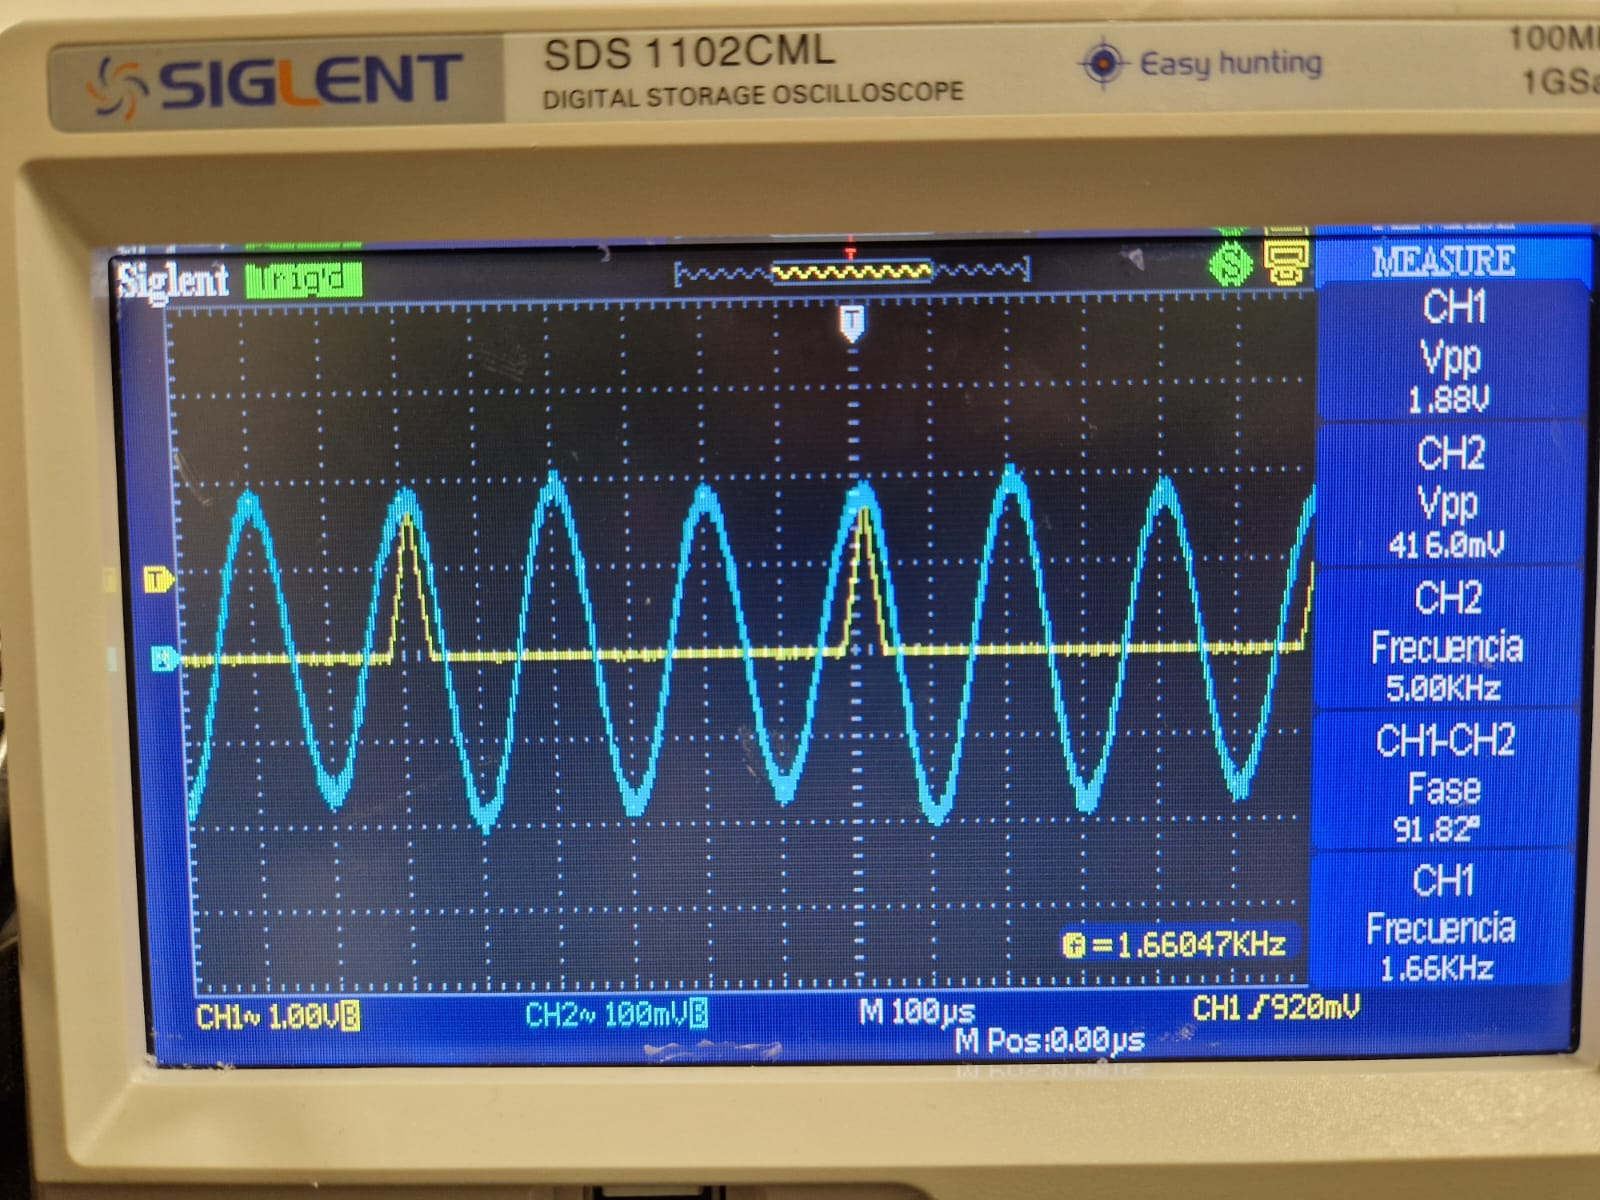
\includegraphics[width=1.05\linewidth]{fourier/delta_dirac/delta3.jpg}
        \subcaption{$n=3$}
        \label{fig:subfig3}
    \end{subfigure}
    \caption{Armónicos correspondientes a $n=1,2,3$}
\end{figure}


\begin{figure}[h!]
    \centering
    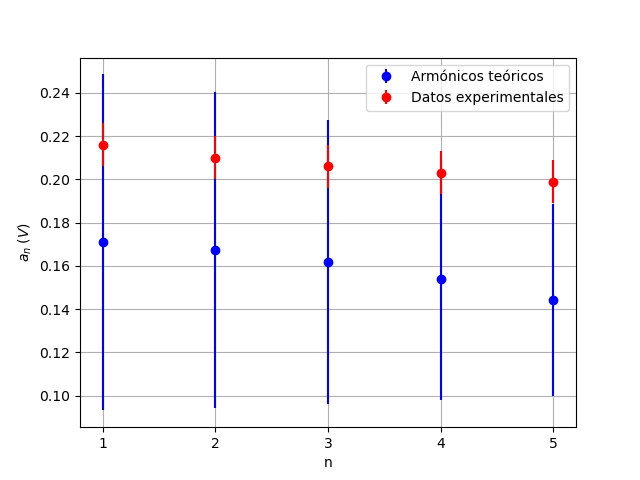
\includegraphics[width=0.55\linewidth]{fourier/pulso_dirac2.png}
    \caption{Armónicos de la delta de Dirac}
    \label{fig:enter-label}
\end{figure}

\newpage

En la figura anterior podemos ver una representación gráfica de los armónicos teóricos y experimentales de nuestro pulso, para comprobar la correlación entre la teoría y los resultados obtenidos en el laboratorio. Una vez realizada la representación gráfica de los resultados resulta más fácil realizar un análisis de la correlación entre los valores teóricos y experimentales. En ambas series de armónicos se puede observar una tendencia clara a decaer ligeramente con $n$, a una velocidad mucho menor que las señales anteriores. No obstante, existe cierta diferencia entre los armónicos teóricos y experimentales, que se mantiene más o menos constante en los armónicos medidos, estando los valores experimentales por encima de los valores teóricos en todo momento. Pese a ser esta diferencia entre los valores muy grande, el resultado experimental de los primeros armónicos entra dentro del rango de incertidumbre de los valores teóricos, que es enorme, llegando a ser casi la mitad del resultado. Esta incertidumbre es tan grande debido a que los coeficientes de Fourier de nuestro pulso dependen de la anchura y del período de la onda, algo que no pasa con las señales anteriores. Estas dos nuevas fuentes de incertidumbre hacen que al realizar la propagación obtengamos incertidumbres casi del mismo orden de magnitud de los propios armónicos teóricos.



\section{Conclusiones}

Para finalizar vamos a realizar un pequeño análisis de los resultados obtenidos, que nos permitirá extraer ciertas conclusiones sobre la precisión y exactitud de nuestro experimento.

En primer lugar vamos a destacar los satisfactorios resultados obtenidos con la señal cuadrada y la triangular, ajustándose los resultados medidos en el laboratorio a los calculados a partir del desarrollo en serie de Fourier de la forma funcional de la señal. Además de eso se ve claramente el comportamiento que siguen los armónicos en función de $n$, siendo los armónicos pares nulos en ambas señales y decayendo los impares según $1/n$ y $1/n^2$ en la onda cuadrada y en la triangular respectivamente. De esta forma podemos concluir que los resultados obtenidos para estas dos ondas tienen tanto una gran precisión como una gran exactitud.

Por otro lado, la otra señal analizada fue el pulso con forma de delta de Dirac. En este caso los resultados experimentales no se corresponden tanto con los valores teóricos, como ya comentamos tras la exposición de nuestras medidas. Los resultados son bastante precisos, pues reflejan de una forma bastante correcta la tendencia que siguen los armónicos en función de $n$, pero carecen de exactitud, ya que en todos los $a_n$ medidos hay una gran diferencia con los valores teóricos. No obstante, estas pequeñas diferencias son comprensibles, ya que durante esta última parte de la práctica las incertidumbres aumentaron radicalmente, como ya mencionamos antes. A las incertidumbres ya comentadas asociadas a la forma funcional de la propia onda debemos sumarle las incertidumbres que el rectificador pudo aportar, que no fueron tenidas en cuenta. Además de eso cabe destacar que en este apartado estuvimos trabajando siempre sobre una gran aproximación, ya que la señal que pretendíamos estudiar, la delta de Dirac, es un pulso infinitamente alto y infinitamente estrecho imposible de reproducir en el laboratorio, que tuvo que ser aproximada por una señal triangular modificada convenientemente.

\newpage

\section{Bibliografía}

\begin{itemize}
    \item \textbf{Edminister, J. A.} \textit{Circuitos eléctricos}. 2a edición. (1994) McGraw-Hill
    \item \textit{Quality factor: Q Factor Formula»Electronics Notes}. https://www.electronics-notes.com\newline/articles/basic\_concepts/q-quality-factor/basics-tutorial-formula.php
    \item \textit{Bandwidth of LCR circuit}. (s.f.). Physics Stack Exchange.https://physics.stackexchange.com\newline/questions/753684/bandwidth-of-lcr-circuit
    \item Guiones de prácticas/Práctica 3: Circuito RLC paralelo. Análisis de Fourier
\end{itemize}

\newpage

\section{Anexo: Incertidumbres en el osciloscopio}

Durante toda la práctica las medidas de voltajes y tiempos fueron tomadas con el osciloscopio digital con el que contábamos en el laboratorio. Todas estas medidas vienen acompañadas de sus respectivas incertidumbres, para las que durante la práctica dimos solo su valor numérico, no detallamos la forma en la que fueron calculadas. El objetivo de este apartado es detallar el procedimiento seguido para calcular estas incertidumbres.

En primer lugar, partimos de que el osciloscopio tiene una resolución, tanto para los voltajes como para los tiempos, que resulta ser variable y podemos ajustar antes de tomar las medidas. Además de eso debemos notar que la pantalla del osciloscopio está dividida en cuadrículas, cuyas líneas verticales y horizontales están a su vez subdivididas. En la siguiente figura podemos apreciar mejor estas divisiones:

\begin{figure}[h!]
    \centering
    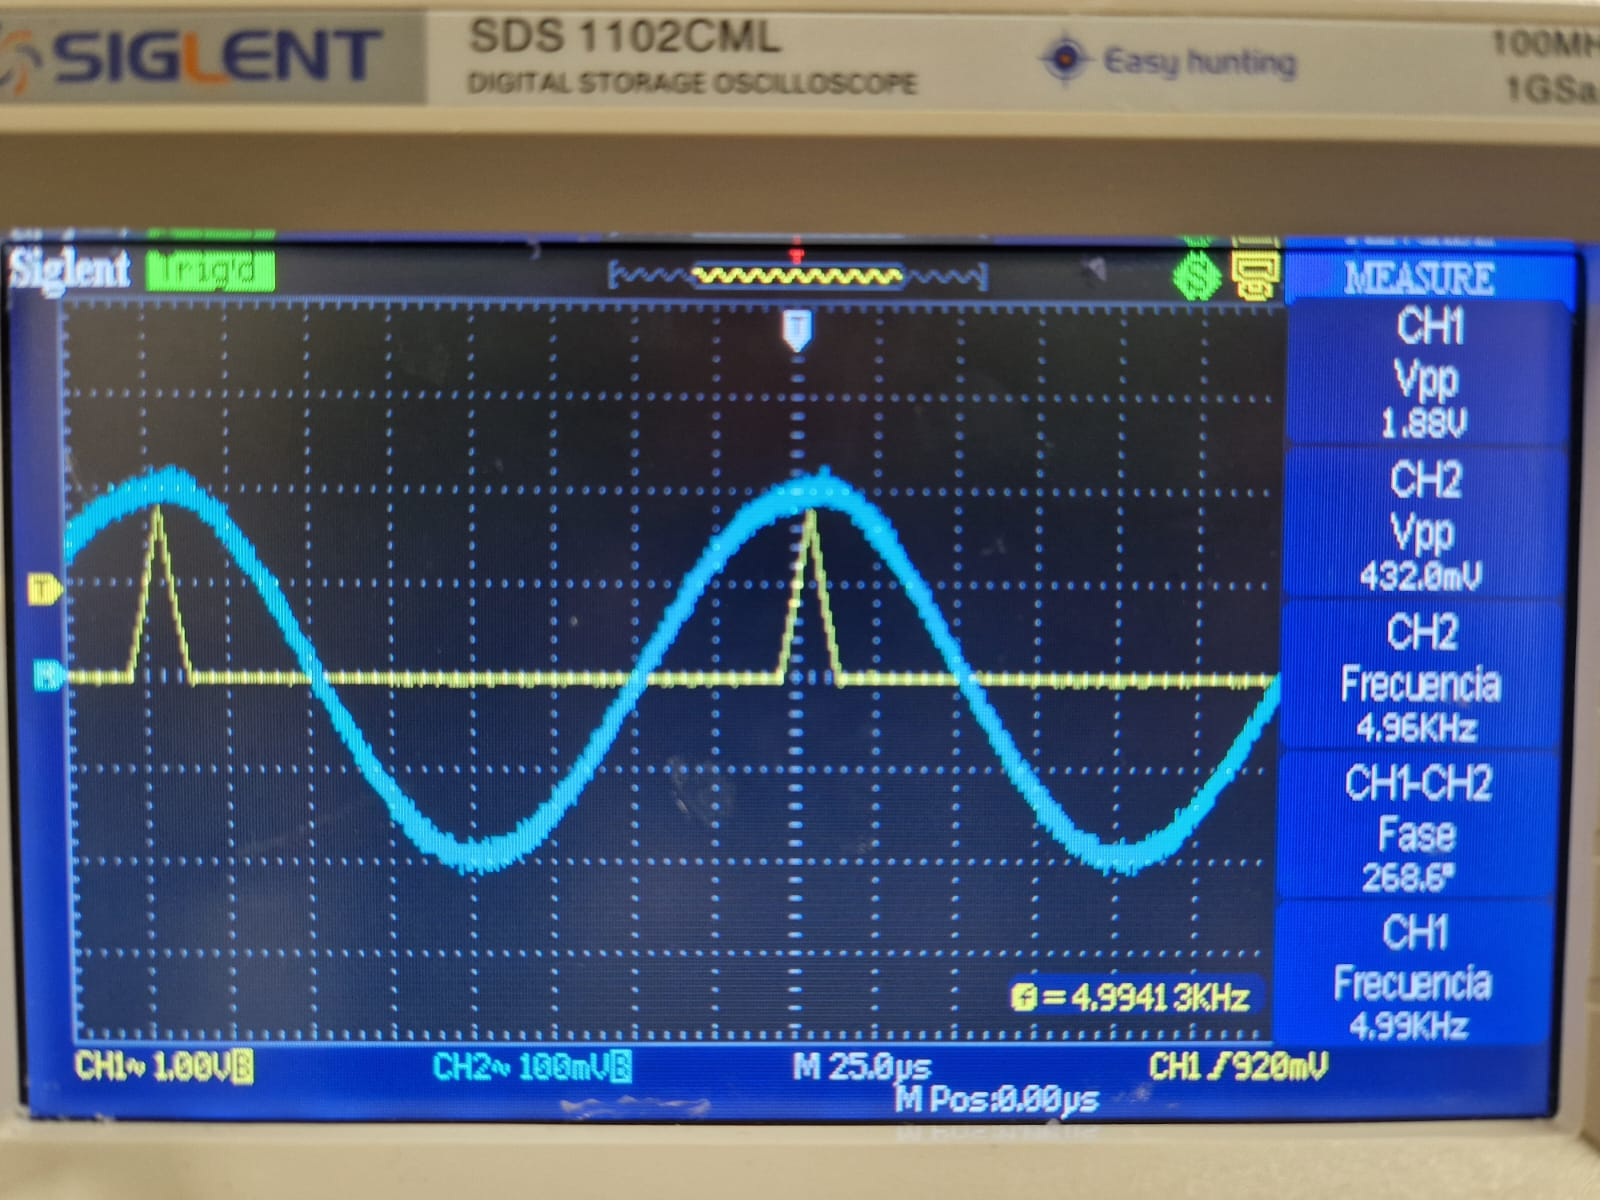
\includegraphics[width= 0.65\linewidth]{fourier/delta_dirac/delta1.jpg}
    \caption{Ejemplo de medida con el osciloscopio}
    \label{fig:enter-label}
\end{figure}

Podemos ver que en nuestro osciloscopio la subdivisión mínima es de 0,2 divisiones, hay cinco divisiones en cada cuadrícula, tanto verticales como horizontales. Además de eso para calcular la resolución es necesario conocer la escala con la que mide el osciloscopio, que aparece en la parte de abajo de la pantalla. Las resoluciones de las medidas de voltajes, las verticales, se corresponden con CH1 y CH2, siendo CH1 la señal de entrada y CH2 la salida. Por otro lado las resoluciones de las medidas temporales son las que corresponden a una $M$, que en la figura se miden en $\mu s$. Teniendo en cuenta la escala la resolución mínima se puede calcular de manera muy sencilla con una multiplicación, por ejemplo para la señal de entrada de la figura la resolución es de:

\begin{equation}
    \delta V = 0,2\;div \cdot 1,00 \;\frac{V}{div} = 0,20 \;V
\end{equation}

Esta resolución $\delta V$ coincidirá con la incertidumbre $s(V)$ de nuestras medidas, de igual forma que la incertidumbre de una regla coincide con su resolución.

\end{document}